% Note that the article class does not have chapters.
\documentclass[10pt,twoside,onecolumn,openany]{book}
\usepackage[bg-print]{dnd} % Options: bg-a4, bg-letter, bg-full, bg-print, bg-none.
\usepackage[italian]{babel}
\usepackage[utf8]{inputenc}
\usepackage{multicol}
\usepackage{graphicx}
\graphicspath{ {images/} }

% Start document
\begin{document}
\fontfamily{ppl}\selectfont % Set text font
% Your content goes here
% Comment this out if you're using the article class.
\begin{Large}
\begin{center}
Tutti i contenuti di questo libro sono \textbf{approfondimenti dal carattere onnisciente}, e quindi pensati per essere \textbf{letti solo dal Game Master} e non dai giocatori.\\
\textit{Ringrazio il mio party, i MIM, che mi hanno permesso ed aiutato a sviluppare questo mondo al quale sono molto affezionato.\\Federico Matteoni}
\end{center}
\end{Large}
\pagebreak
\chapter{Premessa}
\begin{large}
Questo libro contiene tutto il sapere, le informazioni, le conoscenze ed il folklore di \textbf{Ocrilia}, il mondo creato collettivamente dalle menti di:
\begin{center}
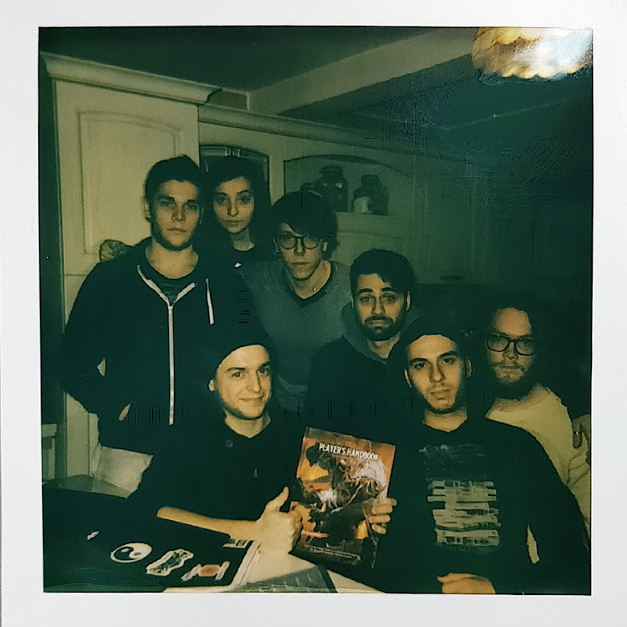
\includegraphics[scale=0.33]{party}
\begin{Large}
\emph{
	\begin{multicols}{3}
		Andrea di Ricco \\
		Samuele Torrigiani \\
		Emanuele Moriconi \\
		Stefano Moriconi \\
		Giuseppe Gatto \\
		Ilaria Battaglia \\
	\end{multicols}
	\begin{multicols}{3}
		\[\:\] \\
		Federico Matteoni \\
		\[\:\] \\
	\end{multicols}
}
\end{Large}
\end{center}
\end{large}
\begin{center}
\includegraphics[scale=0.33]{Ocriliasymbol}
\end{center}
Tutto quello che è contenuto in questa enciclopedia è stato creato giocando a \textbf{Dungeons \& Dragons 5e}, quindi eventuali statistiche o tecnicismi sono da intendersi relativi a quel set di regole. Ambientazione, luoghi e personaggi possono comunque essere usati per un qualsiasi gioco di ruolo o per una qualsiasi storia.\\
Il materiale qui contenuto è \textbf{liberamente utilizzabile per opere personali purché esse siano rilasciate gratuitamente}, a patto di \textbf{riconoscere come autori le persone sopra indicate}.\\
La campagna di Ocrilia è iniziata il 27 Settembre 2016, concludendosi il 12 Febbraio 2018.\\
La trascrizione, l'impaginazione e le informazioni qui contenute sono a cura di \textit{Federico Matteoni}.\\
\newpage
\begin{multicols}{2}
\tableofcontents
\end{multicols}
\pagebreak
\chapter{Cronistoria}
\begin{quotebox}
	"\textit{Si narra che, nei tempi antecedenti la magia, ci fu un boato nel cielo che irrorò il mondo}."\\ \textbf{La Storia dei Tre Maghi}
\end{quotebox}
\begin{multicols}{2}
\begin{itemize}
\itemsep-1em
\item 5989 MIN Viene ufficialmente fondata la città di \textbf{Silandell}.\\
\item 5867 MIN Uno sconosciuto \textbf{raggio di energia} partito dalla collina centrale (più precisamente dalla \textbf{scultura dodecagonale}, ma i locali non sapevano della sua esistenza) scatena un terremoto che rade al suolo la città e mette in fuga gli abitanti.\\
Il luogo verrà considerato maledetto e non verrà mai più abitato.\\
\item 3000 MIN Data a cui tradizionalmente viene fatta iniziare la storia, con la \textbf{scoperta del potere magico}. Si dice sia la data in cui viene ritrovato il \textbf{Maginomicon}.\\
\item 2985 MIN Viene fondata la città di \textbf{Nevreat} da parte di minatori nanici radunati nei dintorni. La città acquisterà rapidamente imponenza e prestigio grazie alla ricchezza ed alla grandiosità delle opere che contiene.\\
\item 2965 MIN Viene fondata la \textbf{Scuola di Magia di Wexria}.\\
\item 2876 MIN Viene istituito l'\textbf{Impero di Venec}\\
\item 2800 MIN Attorno a \textbf{Wexria} viene fondata la città di \textbf{Hellisdalk}, sulla punta della \textbf{Penisola dell'origine}.\\
\item 2796 MIN Viene fondato \textbf{Borgo Legnodoro} in un bosco caratteristico, nell'Ovest di Aluxias.\\
\item 2788 MIN Inizia la \textbf{Guerra degli Eterni}.\\
Gli \textbf{Umani} dell'\textbf{Impero di Venec}, gli \textbf{Elfi} della \textbf{Repubblica di Alosrin} e i \textbf{Nani} dell'\textbf{Impero di Nevreat} si fronteggeranno per ottenere il dominio su tutta \textbf{Aluxias} per molti secoli. Il nome deriva dalla credenza che i capi delle tre fazioni, cioè Alosrin, Nevreat e Venec, fossero sempre in vita e sempre al comando durante tutti i secoli di guerra.\\
\item 1582 MIN Armistizio e divisione dei territori di Aluxias tra le tre fazioni. Proclamazione della \textbf{Coalizione Alosrin-Venec-Nevreat}.\\
\item 1580 MIN \textbf{Attacco di Alder}. Alder, uno stregone che successivamente verrà associato agli \textbf{Obscurant}, evoca un esercito di non-morti che viene annientato da un'armata formata dalla recente coalizione Alosrin-Venec-Nevreat.\\
\item 1230 MIN Inizio della \textbf{Guerra di Dominazione Venec}.\\ L'esercito Venec si scontra contro quello Alosrin dopo secoli di tensioni e provocazioni.\\
\item 1228 MIN L'esercito di Nevreat scende in campo e la Guerra di Dominazione Venec entra nel fulcro.\\
\item 1170 MIN Una coalizione Alosrin-Nevreat sconfigge e si spartisce i territori del defunto Impero Venec. Gli umani, ora inglobati nelle società di nani ed elfi, col tempo vengono accettati e iniziano a nascere le prime \textbf{razze meticce}.\\
\item 1003 MIN Un \textbf{asteroide} precipita nell'oceano a Sud-Est di Aluxias. L'impatto forma quello che diverrà l'\textbf{Arcipelago dei 5 Castelli}. \\
\item 970 MIN - Nel giro di pochi anni delle \textbf{ribellioni umane} scoppiano all'interno dei territori elfici e nanici.\\
\item 960 MIN - Le ribellioni confluiscono e si organizzano nel \textbf{Secondo Impero Venec}.\\
\item 857 MIN - Faide e dissidi all'interno del Secondo Impero Venec ne causano la scissione: nascono il \textbf{Regno di Polig} e la \textbf{Repubblica di Primel}.\\
\item 734 MIN - Un demone gargantuesco viene evocato da una setta di maghi e stregoni cultori delle arti oscure e di un antico mago di nome \textbf{Manvius Dexidas}: si fanno chiamare \textbf{Obscurant} e rivelano di essersi formati agli albori degli studi magici.\\
Il demone viene sconfitto da un umano sconosciuto, che lo imprigionerà sfruttando un potere magico antico e dalle origini ignote.\\
\item 575 MIN - Scoppia la \textbf{Peste Rossa}. In 5 anni la popolazione di Aluxias e Deidras viene \textbf{ridotta al 10\%}. \\
\item 550 MIN - Dopo anni di ricerche congiunte di druidi, maghi e stregoni di ogni razza, viene \textbf{trovata una cura} alla peste rossa: si scopra la sua origine di natura magica.\\
\item 500 MIN - La peste rossa viene \textbf{considerata ufficialmente debellata}.\\
\item 386 MIN - Un'esplosione di origini sconosciute scuote il terreno per ore, provocando disastri che fanno preannunciare la fine del mondo. Proviene dall'estremo Nord-Est e viene distintamente udita da ogni persona.\\
\item 325 MIN - Degli esploratori trovano un antichissimo \textbf{prisma} sotto una collina nel Sud di Aluxias, dal quale trae nutrimento un \textbf{gigantesco albero millenario}. Il luogo viene dichiarato \textbf{inviolabile} e l'albero viene chiamato "\textbf{L'Albero della Creazione} dai pellegrini e gli studiosi magici.\\In pochi anni, dagli accampamenti dei pellegrini si forma una vera e propria città che verrà chiamata \textbf{Riposo del Viandante}.\\
\item 315 MIN - Il team di esploratori responsabile della scoperta del prisma dedica gli anni successivi al ritrovamento e allo studio di \textbf{altre 6 sculture simili} in altrettanti luoghi di entrambi i continenti. Ogni scultura ha proprietà diverse e i luoghi vengono tenuti nascosti.\\
\item 200 MIN - Nei decenni precedenti, in entrambi i continenti si è formato un crescente bisogno di conoscenza e innovazione: con questa data si dà tradizionalmente inizio all'\textbf{Epoca del Rinascimento}. In pochi decenni vengono creati e scoperti milioni tra incantesimi, oggetti magici e pozioni.\\
\item 98 MIN - Un esercito di \textbf{decine di miliardi di non-morti} attacca le principali città e i principali centri abitati. Inizia quella che verrà ben presto chiamata "\textbf{Guerra di Sopravvivenza}".\\
\item 80 MIN - In pochi anni di guerra le perdite sono già numerosissime per la neoformata \textbf{Coalizione Aluxiana}.\\
\item 5 MIN - Hellisdalk, capitale della coalizione aluxiana, viene \textbf{conquistata} e \textbf{quasi completamente rasa al suolo}. I vertici nemici scendono in campo e si presentano per la prima volta: \textbf{sono gli Obscurant}.\\
\item 0 - Una \textbf{Squadra di Elite} della coalizione \textbf{riconquista Hellisdalk} e pone fine alla guerra uccidendo gli ultimi obscurant.\\
Viene dichiarata \textbf{eterna amicizia e collaborazione fra le razze} e viene fondato l'\textbf{Impero Aluxiano}.\\
\item 3 - Inizia la ricostruzione di Hellisdalk: viene progettata affinché il suo aspetto rispecchi la forza e la grandezza della cooperazione.\\
\item 102 - Innumerevoli draghi iniziano a comparire ed attaccare varie parti di entrambi i continenti, portando distruzione. Si formeranno tante squadre indipendenti di \textbf{cacciadraghi} che risolveranno la situazione in pochi decenni.\\
\item 126 - \textbf{Tong'har} viene fondata.\\
\item 131 - Nasce \textbf{Masegroth} ed l'omonimo mercato.\\
\item 630 - Tong'har e Masegroth si staccano dall'impero aluxiano, dichiarandosi indipendenti.\\ Pochi mesi dopo, \textbf{Stellamarina} fa la stessa cosa.\\
\item 753 - Un misterioso naufragio avviene a largo di \textbf{Amareos}: \textbf{il relitto non verrà mai ritrovato}. Circa due mesi dopo, un'eclissi di origine sconosciuta \textbf{oscurerà Ontalia per circa tre ore}.\\ \textit{Questo è l'anno nel quale si colloca questa enciclopedia}.\\
\end{itemize}
\end{multicols}
\newpage
\chapter{Ocrilia}
\begin{center}
\includegraphics[scale=0.8]{quriaocriliapianeti1}
\end{center}
\begin{multicols}{2}
\paragraph{Ocrilia e Quria} \textbf{Ocrilia} è il satellite naturale di una \textbf{superterra} che prende il nome di \textbf{Quria}, orbitante intorno ad una stella della sequenza principale che gli ocriliani hanno chiamato \textbf{Ontalia}.\\
\textbf{Ocrilia} è un frammento di \textbf{Quria} spaccatosi in seguito ad un impatto con un planetoide avvenuto circa \textbf{5 miliardi di anni fa}. \textbf{Quria} è una realtà molto diversa rispetto ad \textbf{Ocrilia}: su questa superterra dalla profonda cicatrice la vita si è sviluppata molto prima. Di \textbf{Quria} verrà, forse, trattato in un'altra enciclopedia.
\columnbreak
\subparagraph{Perché Quria} \textbf{Quria} è il nome dato dagli indigeni ocriliani alla Dea che ha generato la realtà: l'universo, che prende il nome di \textbf{Orbìtio}, la vita, \textbf{Ocrìlia}, la luce, chiamata \textbf{Ontàlia}, e tutto quanto in essi. Il nome \textbf{Ocrilia}, quindi, sta al satellite naturale come il nome \textbf{Gaia} sta alla Terra.
\end{multicols}
\paragraph{Cos'è Ocrilia} \textbf{Ocrilia} è un satellite naturale in orbita sincrona con \textbf{Quria}: rivolge sempre la stessa faccia alla superterra, quella "inferiore" simile ad un cumulo di macerie protratto verso di essa. L'altra faccia, dove la vita si è sviluppata, è quasi piatta e dai bordi frastagliati. Le bussole rispondono al campo magnetico di Quria. L'orbita è sul piano dell'equatore e non risente di variazioni durante la rivoluzione, che dura 24h.\\
\newpage
\section{Il Tempo}
\paragraph{Come suddividono il tempo gli Ocriliani?}
A causa dell'assenza di una luna o di qualsivoglia satellite naturale, non esiste il concetto di \textbf{mese} per gli abitanti di \textbf{Ocrilia}. Loro, invece, suddividono l'anno, che è di 380 giorni (calcolati dall'astronomo \textbf{Hiram Mallin} circa nel 2980 MIN, sulla base di osservazioni stellari) in 10 \textbf{MAL} da 38 giorni ciascuno. Questa suddivisione naturale dell'anno in \textbf{dieci parti} è stata suggerita dal \textbf{Mallin} stesso sulla base delle \textbf{cinque stagioni} che passano durante l'anno. Tradizionalmente, il nome del MAL e quello della stagione sono scritti insieme quando si riporta una data, es. \textit{lo Zel dodicesimo della Prateria Luminosa}.\\
Le cinque stagioni sono:
\begin{multicols}{2}
\begin{itemize}
\item \textbf{Rinata}, la stagione della fioritura e dell'innalzamento delle temperature
\item \textbf{Luminosa}, il calore raggiunge i picchi massimi e le paludi si ritirano
\item \textbf{Vecchia}, i fiori appassiscono e le foglie ingialliscono
\item \textbf{Silenziosa}, le rigide temperature e l'ovattamento della neve rendono ogni suono più lieve
\item \textbf{Ripresa}, le nevi si ritraggono e la natura torna a respirare
\end{itemize}
\end{multicols}
I nomi dei MAL sono ispirati agli eventi significativi che avvengono a inizio e a fine stagione. Essi sono, riportati in ordine con l'elenco precedente:
\begin{multicols}{2}
\begin{itemize}
\item \textbf{Fioritura}, le piante tornano ad essere rigogliose
\item \textbf{Temperatura}, la temperatura sale e torna calorosa
\item \textbf{Prateria}, l'erba torna fresca e rigogliosa
\item \textbf{Sabbia}, spiaggia e mare sono di nuovo accoglienti
\item \textbf{Pianta}, i rami seccano e le foglie cadono
\item \textbf{Tana}, gli animali per lungo tempo dormono
\item \textbf{Città}, le piazze lentamente si svuotano
\item \textbf{Tundra}, boschi e praterie velocemente s'imbiancano
\item \textbf{Prima}, la fauna pian piano dalla tana esce fuori
\item \textbf{Seconda}, la natura come sempre torna agli albori
\end{itemize}
\end{multicols}
Ogni MAL è suddiviso quattro blocchi di 8 giorni, di cui 7 lavorativi ed 1 festivo, ed i 6 giorni rimanenti sono tradizionalmente adibiti a festa, studio, e altre attività personali.\\
Gli 8 \textbf{giorni comunitari} hanno nomi tratti da rune antiche che simboleggiano la semplicità:
\begin{multicols}{2}
\begin{itemize}
\item \textbf{Lot}, luce
\item \textbf{Kib}, onda
\item \textbf{Jep}, fuoco
\item \textbf{Zel}, campo
\item \textbf{Tai}, acqua
\item \textbf{Mes}, cielo
\item \textbf{Rok}, aria
\item \textbf{Dul}, musica, giorno festivo
\end{itemize}
\end{multicols}
mentre i rimanenti 6 \textbf{giorni personali} sono chiamati in onore di grandi personaggi del passato:
\begin{multicols}{2}
\begin{itemize}
\item \textbf{Keylee}, la leader degli \textbf{Elite}, \textbf{trentatresimo} giorno
\item \textbf{Folmin}, degli \textbf{Elite}, \textbf{trentaquattresimo} giorno
\item \textbf{Lotho}, degli \textbf{Elite}, \textbf{trentacinquesimo} giorno
\item \textbf{Thocero}, degli \textbf{Elite}, \textbf{trentaseiesimo} giorno
\item \textbf{Kherrah}, degli \textbf{Elite}, \textbf{trentasettesimo} giorno
\item \textbf{Hiram}, che ha ideato e progettato il calendario, in segno di rispetto, \textbf{trentottesimo} giorno
\end{itemize}
\end{multicols}
%L K J Z T M R D  L K J Z T M R D  L K J Z T M R D  L K J Z T M R D  K F L T K H
\includegraphics[scale=0.735]{days}
\pagebreak
\paragraph{Date storiche} Secondo la tradizione imperiale dell'attuale \textbf{Impero Aluxiano}, le date vengono scandite a partire dall'anno della \textbf{riconquista di Hellisdalk}, diventato l'anno 0. Alle date precedenti, contate alla rovescia fino all'anno 0, viene aggiunto il suffisso \textbf{MIN}, che significa \textit{prima}: non è specificato prima di cosa, ogni \textbf{aluxiano} e \textbf{deidriano} conosce bene gli avvenimenti che hanno distinto la \textbf{Guerra di Sopravvivenza}. Alle date successive può essere aggiunto il suffisso \textbf{AP}, cioè \textit{dopo}, ma non viene usato.\\
Secondo gli storici, \textbf{Hellisdalk} venne liberata il \textbf{Mes quattordicesimo della Fioritura Rinata}.\\
\subparagraph{Prima della Guerra di Sopravvivenza} Ad \textbf{Aluxias} e \textbf{Deidras} si sono adottati modi diversi per specificare le date nel corso dei millenni.\\
In ordine cronologico:
\begin{itemize}
\item \textbf{Silandell}, e il resto di \textbf{Deidras}, contava le proprie date a partire dalla propria fondazione avvenuta nel \textbf{5989 MIN}. La rifondazione di \textbf{Hellisdalk} quindi, secondo il calendario di \textbf{Silandel}, è avvenuta nel \textbf{5989 D.F.}, che sta per \textit{Dopo Fondazione}. La storia di \textbf{Silandell}, però, si è conclusa appena nel \textbf{122 D.F.}.
\item La \textbf{Scuola di Magia di Wexria}, e la comunità magica in generale, contavano gli anni a partire dalla sua istituzione nel \textbf{2965 MIN}. La rifondazione di \textbf{Hellisdalk} quindi, secondo il calendario di \textbf{Wexria}, è avvenuta nel \textbf{Anno degli Studi 2965}.
\item \textbf{Hellisdalk} inizialmente contava gli anni dalla sua prima fondazione, nel \textbf{2800 MIN}. La sua rifondazione è quindi avvenuta nel \textbf{2800 AP}, poiché la stessa nomenclatura è stata riadottata in memoria del passato. La \textbf{Repubblica di Alosrin}, avendo \textbf{Hellisdalk} come capitale, è la fautrice di questo sistema di calcolo delle date.
\item L'\textbf{Impero Venec} monitorava gli anni dalla sua istituzione, avvenuta nel \textbf{2876 MIN}. La \textbf{Guerra degli Eterni}, ad esempio, è scoppiata nell'\textbf{Ottantottesimo Anno dalla Fondazione dell'Impero}.
\item Il \textbf{Secondo Impero Venec}, nato nel \textbf{960 MIN}, riprendeva il conteggio dalla fondazione del primo \textbf{Impero Venec}. La \textbf{Repubblica di Primel} e il \textbf{Regno di Polig} calcolavano gli anni, invece, dalla rispettiva fondazione.
\item \textbf{Nevreat}, la capitale dell'\textbf{Impero di Nevreat}, fu fondata nel \textbf{2985 MIN}. La \textbf{Guerra degli Eterni}, per il popolo nanico di \textbf{Nevreat}, scoppiò quindi nel \textbf{197 Ena}, espressione che significa \textit{dopo}.
\end{itemize}
Stagioni, giorni e mal, invece, sono stati chiamati sempre in maniera diversa ma seguendo sempre la solita filosofia di fondo, data la comodità e la naturalezza con cui essa era stata ideata.
\newpage
\section{Il Cielo}
\paragraph{Nessun satellite naturale} Attorno ad \textbf{Ocrilia} non orbita nessun satellite naturale. Questo comporta notti completamente buie, tetre, dove si può solo fare affidamento sulla luce di fuochi, lanterne e fonti magiche. Inoltre, nelle menti degli ocriliani il concetto di \textit{mese} non si è sviluppato come sulla Terra, dove il ciclo di 27 giorni della Luna è sempre stato usato come punto di riferimento. In assenza di un satellite, gli ocriliani hanno adottato una suddivisione dell'anno molto più semplice: l'hanno diviso in 10, come visto nella sezione precedente.
\paragraph{Costellazioni} Escluso Orbitio, ogni costellazione è associata ad un elemento.
\begin{multicols}{2}
\begin{itemize}
\item \textbf{Orbitio}, 8 stelle disposte a spirale che rappresentano l'universo. Considerato al pari di \textbf{Ocrilia}, essendo suo fratello secondo la tradizione
\item \textbf{Il Pugnale}, 7 stelle. Alla punta del Pugnale appartiene la stella più luminiosa del cielo notturno: \textbf{Ovech}. Associato alla \textbf{Guerra} \textit{nella quale attacca}
\item \textbf{La Falce}, 5 stelle. Associata alla \textbf{Natura} \textit{la quale porta via}
\item \textbf{L'Occhio}, 5 stelle disposte a rombo con una centrale che è anche la pià luminosa. Associato alla \textbf{Conoscenza} \textit{alla quale attinge}
\item \textbf{L'Albero}, 11 stelle a forma di piccolo albero spoglio. Associato alla \textbf{Natura} \textit{la quale fa crescere}
\item \textbf{Il Libro}, 8 stelle disposte a libro aperto. Tra le due pagine c'è una nebulosa facilmente visibile ad occhio nudo che dà l'idea di scritte o di illustrazioni del libro. Associato alla \textbf{Conoscenza} \textit{la quale trasporta}
\item \textbf{Il Corvo}, 10 stelle che formano un volatile stilizzato che sembra scappare dal Gatto. La stella più luminosa forma l'occhio. Associato all'\textbf{Inganno} \textit{con il quale attacca}
\item \textbf{Il Gatto}, 10 stelle che formano un quadrupede stilizzato con la stella più luminosa a formare l'occhio. Sembra inseguire il Volatile. Associato alla \textbf{Vita} \textit{la quale protegge}
\item \textbf{L'Altare}, 4 stelle disposte a trapezio che stilizzano la forma semplice di un \textbf{Altare ad Ocrilia}. Associato alla \textbf{Luce} \textit{la quale venera}
\item \textbf{Il Viandante}, 13 stelle molto vicine che formano la stilizzazione di un umanoide con un bastone. Associato alla \textbf{Tempesta} \textit{dalla quale si protegge}
\item \textbf{Il Demone}, 8 stelle che formano un volto con corna, le cui punte sono le due stelle più luminose. Associato alla \textbf{Morte} \textit{la quale porta}
\item \textbf{L'Ala}, 5 stelle che stilizzano la sagoma di un'ala piumata. Associata alla \textbf{Luce} \textit{la quale porta}
\item \textbf{Il Guanto}, 11 stelle formano un guanto senza dita col mignolo separato dalle altre dita. Associato all'\textbf{Inganno} \textit{con il quale si nasconde}
\item \textbf{L'Osso}, 6 stelle stilizzano un femore umano. Associato alla \textbf{Morte} \textit{la quale segnala}
\item \textbf{Il Fulmine}, 4 stelle formano una saetta stilizzata. Associato alla \textbf{Tempesta} \textit{dalla quale è provocato}
\item \textbf{Lo Scudo}, 6 stelle ad esagono allungato. Associato alla \textbf{Guerra} \textit{nella quale protegge}
\item \textbf{La Culla}, 8 stelle rappresentano una culla rivolta a tre-quarti. Associata alla \textbf{Vita} \textit{la quale annuncia}
\end{itemize}
\end{multicols}
\paragraph{Corpi celesti} Nel cielo notturno punteggiato di stelle, millenni di osservazioni astronomiche grezze hanno individuato un gruppo di stelle non fisse, dai colori singolari e dal moto particolare. Gli ocriliani li hanno interpretati come i \textbf{guardiani} generati da \textbf{Quria} che pattugliano l'universo e vegliano sui tre fratelli: \textbf{Orbitio}, \textbf{Ontalia} e \textbf{Ocrilia}.\\
In realtà essi sono \textit{oggetti} presenti del sistema stellare di \textbf{Ontalia} e sono 8:
\begin{multicols}{2}
\begin{itemize}
\item \textbf{Liatis}, vicino a \textbf{Ontalia} e dalla luce bianca ma sovrastata dalla luce di \textbf{Ontalia}
\item \textbf{Meomia}, dalla forte luce lievemente gialla
\item \textbf{Jieter e Goibos}, un sistema binario. \textbf{Jieter} è di un flebile rosso e \textbf{Goibos} è leggermente azzurro. Ad occhio nudo si riescono a distinguere l'un l'altro solo durante la \textbf{Città Silenziosa}
\item \textbf{Apoth}, dalla luce bianca
\item \textbf{Larak}, la cui luce è leggermente verde
\item \textbf{Ubos}, violaceo
\item \textbf{Zaya}, la più fioca ma dalla luce fortemente rossa
\end{itemize}
\end{multicols}
Ma nel sistema di \textbf{Ontalia} c'è altro che gli ocriliani non sono ancora riusciti a scovare.
\pagebreak
\section{L'Economia}
\begin{multicols}{2}
\paragraph{Rame, Argento, Oro e Platino}
L'economia di \textbf{Aluxias} e \textbf{Deidras} si basa su monete di rame, oro, argento e platino. \textbf{Ogni moneta imperiale} presenta una flebile traccia magica in grado di essere generata solo dai maghi al servizio della \textbf{Zecca Imperiale}. L'ubicazione e il funzionamento della zecca è celata al popolo, garantendone la sicurezza.\\
\begin{commentbox}{{Zecca Imperiale}}
	La \textbf{Zecca Imperiale} si trova sulla \textbf{Penisola dell'Origine}, superata \textbf{La Barriera} in direzione di \textbf{Hellisdalk}, e dopo 17Km di strada, c'è una stradina sulla destra che si dirige verso la costa. L'edificio, simile ad una fortezza, è pattugliato da \textbf{guardie scelte}, recintato a 2Km dalla porta principale e l'accesso è riservato.\\
	Alla zecca vengono trasportate grandi quantità di metalli ogni 15 giorni. All'interno, i 10 maghi incaricati del conio, chiamati \textbf{Sigillatori}, applicano il cosìddetto \textbf{sigillo} sulle monete appena estratte dalla forgia: questo \textbf{sigillo} consiste in un timbro magico unico, cambiato ogni anno, impossibile da riprodurre senza trovarsi all'interno delle stanze predisposte a questa attività.\\
\end{commentbox}
\paragraph{Le Monete} Ogni moneta è decorata con una piccola incisione, che può essere diversa anche per monete coniate nello stesso anno. Di seguito qualche esempio:
\begin{itemize}
\item Molte \textbf{monete d'oro} coniante nell'anno 3 raffigurano un triangolo con un buco al centro, a simboleggiare la neonata \textbf{Coalizione Aluxiana} e la collaborazione delle \textbf{tre razze principali}.
\item Intorno al 550 MIN le \textbf{monete d'oro e d'argento} raffiguravano, in parti diverse dell'anno, profili diversi degli studiosi che hanno trovato la cura alla \textbf{peste rossa}: \textbf{Alinar Morzana, Sarya Quilee, Dalodika Manleggera e Rolim Vensys}.
\item Nel 325 MIN le \textbf{monete d'argento} raffiguravano l'\textbf{Albero della Creazione}.
\end{itemize}
\end{multicols}
\newpage
\chapter{Piano Materiale}
\section{Introduzione}
Ogni luogo di questo mondo, come nel mondo reale, ha una \textbf{storia}, ha \textbf{persone con ricordi legati ad esso}, ha delle \textbf{particolarità}. Ogni città, paese o capanna può nascondere un \textbf{grande tesoro}, o un \textbf{pericolo mortale}. \\
Tutto ciò che esiste in questo mondo è visitabile, \emph{e influenzabile}, da qualsiasi personaggio vivente in esso. \\
I luoghi sono stati pensati per essere visitati secondo una filosofia \textbf{openworld}, perciò si prestano benissimo anche a storie più guidate e con meno libero arbitrio.\\
\begin{center}
\includegraphics[scale=0.75]{AluxiasDeidrastagged}
\end{center}
\newpage
\section{Continenti principali}
\subsection{Aluxias}
Il continente dove si concentrano maggiormente le vicende storiche e da cui è possibile trarre maggiori informazioni.\\ Lo \textbf{Stretto delle Terre} lo separa dal contiente di \textbf{Deidras}.\\
Da \textbf{Amareos} alla longitudine di \textbf{Hellisdalk} sono 330Km in linea d'aria, 420Km fino alla longitudine del punto più orientale di \textbf{Deidras}.\\
Da \textbf{Canalipoli} al punto più meridionale di \textbf{Aluxias}, in linea d'aria sono circa 300Km.
\begin{multicols}{2}
\subsubsection{Città}
\begin{itemize}
\item \textbf{Amareos}, villaggio portuale ad Ovest
\item \textbf{Borgo Legnodoro}, cittadina immersa nei caratteristici \textbf{Boschi Lucenti} ad Est di Amareos
\item \textbf{Canalipoli}, città portuale dai caratteristici canali a Nord del continente
\item \textbf{Riposo del Viandante}, città ai piedi dell'\textbf{Albero della Creazione}, a Sud di Canalipoli
\item \textbf{Pièbianco}, villaggio di minatori e mercanti nella valle più ampia delle \textbf{Rocce di Mezzo} e ai piedi dell'imponente \textbf{Biancacima} al centro del continente
\item \textbf{Stellamarina}, città posta sul delta del fiume \textbf{Dhost}, al culmine delle \textbf{Paludi di R'Lyeh} nell'estremo Sud
\item \textbf{Acqueombrose}, piccolo villaggio a Ovest di Stellamarina, alla sorgente del \textbf{Dhost} e nel mezzo delle \textbf{Paludi di R'Lyeh}
\item \textbf{Acquincrocio}, cittadina ad Est di Stellamarina, sul delta del fiume \textbf{Grhor}
\item \textbf{Hellisdalk}, imponente capitale dell'Impero Aluxiano, posta al culmine della \textbf{Penisola dell'Origine}
\end{itemize}
\columnbreak
\subsubsection{Altri luoghi}
\begin{itemize}
\item \textbf{La Barriera}, massiccia muraglia posta all'istmo da cui parte la \textbf{Penisola dell'Origine}
\item \textbf{Castello di Manvius}, antico e imponente, situato tra le vette innevate delle montagne settentrionali, a Ovest di Canalipoli
\item \textbf{Biancacima}, la montagna più alta delle \textbf{Rocce di Mezzo}, alta più di 10Km
\item \textbf{Casa di Duan}, un casolare abitato da monaci combattenti sulle \textbf{Rocce di Mezzo} a Sud delle \textbf{Paludi di R'Lyeh}
\end{itemize}
\begin{commentbox}{{Etimologia}}
Tratti da lingue antiche e rimasti nella tradizione, i nomi dei continenti hanno significati importanti. \textbf{Aluxias} significa \textit{Terra Madre}, mentre \textbf{Deidras} si traduce in \textit{Terra Figlia}.
\end{commentbox}
\end{multicols}
\subsection{Deidras}
Più piccolo di \textbf{Aluxias}, la sua morfologia è nettamente divisa in una zona boschiva, il \textbf{Verdebosco}, a Ovest, e in una zona collinare e montana a Est, i \textbf{Sassi Orientali}.
\begin{multicols}{2}
\subsubsection{Città}
\begin{itemize}
\item \textbf{Masegroth}, città portuale sede dell'omonimo fiorente mercato, a Nord del continente
\item \textbf{Tong'har}, città incastonata nella roccia dei \textbf{Sassi Orientali}, a Sud di Masegroth
\end{itemize}
\columnbreak
\subsubsection{Altri luoghi}
\begin{itemize}
\item \textbf{Silandell}, antica città in rovina e popolata di mostri ed altri pericoli nel Sud del continente
\item \textbf{Cripta del Desiderio}, labirintiche rovine dove, secondo le leggende, si trova un \textbf{Pozzo dei Desideri}, a Est di \textbf{Tong'har}
\end{itemize}
\end{multicols}
\newpage
\subsection{Arcipelago dei Cinque Castelli}
Arcipelago di quattro isole che prende il nome dalle \textbf{cinque rovine} sparse per l'arcipelago.
\begin{multicols}{2}
\subsubsection{Città}
\begin{itemize}
\item \textbf{Melar}, villaggio di pescatori e barcaioli a Ovest
\item \textbf{Nassau}, cittadina libera di pirati e banditi, a Est
\end{itemize}
\begin{commentbox}{{Origine}}
L'Arcipelago dei Cinque Castelli si è generato in seguito all'\textbf{impatto di un asteroide}, avvenuto nel \textbf{1003 MIN}.
\end{commentbox}
\columnbreak
\subsubsection{Altri luoghi}
\begin{itemize}
\item \textbf{Borgo Fantasma}, a Sud Ovest
\item \textbf{Torre Infinita}, a Sud Est
\item \textbf{Castello di Strahd}, a Sud di \textbf{Melar}
\item \textbf{Cancello per gli Inferi}, a Sud di \textbf{Nassau}
\item \textbf{Dimora di Kwalish}, al centro dell'arcipelago
\end{itemize}
\end{multicols}
\subsection{Ulan}
Continente all'estremo Nord-Est di \textbf{Aluxias} e \textbf{Deidras}, prossimo al bordo di \textbf{Ocrilia}. Quasi interamente disabitato, esclusa una piccola comunità nell'entroterra, è totalmente sconosciuto agli abitanti di \textbf{Aluxias} e \textbf{Deidras}. La sua gigantesca pianura è abitata da mostri e creature enormi e pericolose. Lungo tutte le coste rocciose si possono trovare i relitti di navi da antichissime a recenti.\\
\begin{multicols}{2}
\subsubsection{Città}
\begin{itemize}
\item \textbf{Villaggio di Ulan}, al centro del continente ed immerso nella prateria circostante
\end{itemize}
\columnbreak
\subsubsection{Altri luoghi}
\begin{itemize}
\item \textbf{Cratere}, provocato da un'esplosione nel 386 MIN di "\textit{origini sconosciute}".
\end{itemize}
\end{multicols}
\begin{center}
\includegraphics[scale=0.75]{Ulan}
\end{center}
\newpage
\section{Città, paesi e villaggi nel dettaglio}
\subsection{Amareos}
Questo villaggio ha iniziato a formarsi in antichità dagli accampamenti dei pescatori insediati nei paraggi. Dal \textbf{2800 MIN} circa in poi il luogo è diventato uno scalo importante per il traffico locale, evolvendosi in pochi anni e diventando molto frequentato da mercantili e navi passaggeri: nonostante la dimensione, è \textbf{lo scalo più importante dell'Aluxias occidentale}.\\
La città è composta da pochi edifici d'interesse, ma da molte capanne e abitazioni. Durante l'anno la densità demografica varia molto, passando da diverse centinaia di persone durante la primavera-estate a poche decine durante l'autunno-inverno quando il traffico marittimo è minore.\\
\\
\includegraphics[scale=0.6]{Amareos}
\subsubsection{Storia}
Già intorno al 2900 MIN in questa zona era presente un piccolo molo di fortuna costruito dai pescatori locali per facilitarsi la vita. Col tempo e l'aumento demografico l'insediamento attorno al molto è cresciuto, molto lentamente, fino a diventare delle attuali dimensioni.\\
Intorno al 2670 MIN un'armata Nevreat ha presidiato il luogo, che era sotto il controllo dell'Impero di Nevec. Durante il periodo di occupazione il villaggio si è svuotato ed è andato in rovina. Rimane disabitato fino al 1170 MIN circa, quando l'Impero di Nevreat ottiene il controllo della zona e ricostruisce il molo. Ritornata nelle mani umane con la forza nel 960 MIN, passerà poi al Regno di Polig che la sfrutterà come molo per i propri traffici fino allo scoppio della \textbf{Guerra di Sopravvivenza}.\\
Inizia a ritornare abitata dall'8 circa, venendo lentamente ricostruita e tornando all dimensioni di un tempo.
\newpage
\subsubsection{Luoghi}
\begin{multicols}{2}
\paragraph{Magazzino}
Dentro questo edificio di medie dimensioni si trovano stoccate tutte le merci che passano dalla città, in attesa di essere caricate su una carovana o una nave.\\
L'edificio funge da vero e proprio centro di scambio della città, con qualche mercante che lo sfrutta per vendere la propria merce.\\ Il sovrintendente è anche la persona più importante della città, assumendo \textit{de facto} il ruolo di governatore. Attualmente è l'umano \textbf{David Brethel}.
\columnbreak
\begin{paperbox}{{David Brethel}}
	Giovane, di bell'aspetto, muscoloso e alto, \textbf{David Brethel} è il classico esempio del gradasso pieno di sé. Gestisce le merci, gli scambi e, \textit{de facto}, la città in maniera giusta e corretta, ma sempre strizzando l'occhio agli interessi suoi e dei suoi collaboratori. Ha due guardie del corpo che lo venerano e rispondono ad ogni suo ordine, i gemelli mezzorchi \textbf{Zeth} e \textbf{Eset}.
\end{paperbox}
\end{multicols}
\begin{multicols}{2}
\paragraph{Scudiero}
L'halfling \textbf{Berengar Zoccoferro}, con la moglie \textbf{Rutilde} e il figlioletto \textbf{Malaric}, si occupano di sistemare le carovane e nutrire i cavalli portati in città. L'edificio ha abbastanza spazio per una decina di cavalli, oltre ad essere la casa della famiglia Zoccoferro.\\
\textbf{Servizi offerti}
\begin{dndtable}
   	\textbf{Servizio}  & \textbf{Costo} \\
   	Cavallo leggero & 75 mo \\
   	Stallaggio & 5 ma / giorno \\
   	Carovana & 100 mo
\end{dndtable}
\end{multicols}
\begin{multicols}{2}
\begin{paperbox}{{Berengar Zoccoferro e famiglia}}
	\textbf{Berengar} è un halfing caloroso e gentile, sempre pronto ad aiutare ma non incline a fare sconti ai primi arrivati. Offre sempre da bere a trattazioni concluse e spesso lo si trova indaffarato, intento a concludere una riparazione o a riempire le ciotole di biada per i cavalli.\\
	La moglie \textbf{Rutilde} è anch'essa molto gentile ma più distaccata e coglie la prima occasione per lasciare gestire i clienti al marito, preferendo il lavoro nel retrobottega o nella contabilità.\\
	\textbf{Malaric} è ancora giovane ma molto energico, instancabile aiutante dei genitori ma non appena un cliente gli dà corda si perde in giochi e scherzi.\\
\end{paperbox}
\columnbreak
\begin{commentbox}{{Consiglio}}
\textbf{Berengar} può essere distratto da un cliente particolarmente insistente o un cavallo imbizzarrito e non accorgersi di una ripulita al forziere che tiene dietro il bancone.\\
Però neanche si pone delle domande riguardo i cavalli che accoglie, sulla loro \textit{rarità} o su eventuali selle o accessori \textit{insoliti e dai poteri magici}.\\
\end{commentbox}
\end{multicols}
\begin{multicols}{2}
\paragraph{Locanda "La Visione Marina"}
Gestita da una mezzelfa alla mano di nome \textbf{Calarel Lliamenor}, questa locanda spaziosa e aperta su tutti e quattro i lati ha una terrazza liberamente accessibile dalla quale si può godere di una meravigliosa vista sull'oceano, specialmente al tramonto.\\
\textbf{Servizi offerti}
\begin{dndtable}
	\textbf{Servizio} & \textbf{Costo} \\
	Boccale di birra & 1 ma \\
	Liquore di squalo & 5 ma \\
	Pasto medio & 1 mo \\
	Pasto abbondante & 3 mo \\
	Stanza & 5 ma / notte \\
\end{dndtable}
\begin{paperbox}{{Calariel Lliamenor}}
	\textbf{Calariel} è una mezzelfa dai capelli ramati e dal viso tempestato di lentiggini, molto energica e alla mano. Ama la vita in questa locanda frequentata da marinai, le feste spontanee che nascono e gli incontri felici in cui si concludono. Viene da una famiglia prevalentemente di umani che le hanno dato il lato festaiolo. La parte elfica le ha donato l'aspetto elegante e la bellezza mozzafiato, ma non la diffidenza. Può essere troppo irriverente e sconsiderata, rischiando di oltrepassare il confine troppo spesso.
\end{paperbox}
\end{multicols}
\newpage
\begin{multicols}{2}
\paragraph{Fabbro}
Piccola bottega di \textbf{Grerg}, il mezzorco fabbro che amorevolmente la gestisce. L'edificio è molto piccolo, giusto lo spazio della fucina, un paio di tavoli, il bancone ed una rastrelliera dietro esso, semivuota in cui più che altro vengono riposte le armi in consegna per essere riparate.\\
\begin{paperbox}{{Grerg}}
	Il mezzorco \textbf{Grerg} ha un temperamento semplice, non brilla per intelligenza nè per bravura, ma è apprezzato per la dedizione che mette nel suo lavoro e la puntualità delle sue consegne. Inoltre, ai clienti affezionati fa ottimi prezzi. Ha sempre abitato in città e conosce bene i dintorni.\\
\end{paperbox}
\end{multicols}
\begin{multicols}{2}
\begin{quotebox}
"\textit{Anni fa uno strambo nano aveva l'abitudine di pescare lanciando saette dal Molo Dritto e strinando tutti i pesci dei dintorni. Fu pestato da un gruppo di marinai, non l'ho più visto da allora...}."\\ \textbf{Elred Reynorin}, un anziano elfo del luogo.
\end{quotebox}
\columnbreak
\paragraph{Molo}
Sorvegliato da volontari, il molo è facilmente accessibile dalla via centrale della città.\\
Il molo centrale, chiamato \textbf{Molo Dritto} dai locali, è dedicato alle imbarcazioni dal grosso tonnellaggio come galeoni e fregate. Ne supporta quattro o cinque, se ben ancorate.\\
Il molo secondario, \textbf{Molo Storto}, è per pescherecci e barche passeggere piccole o medie. Può supportare tra le 20 e le 40 imbarcazioni.\\
\end{multicols}
\paragraph{Piazza Centrale}
Lo spiazzo centrale di Amareos è frequentato dai vari mercanti che sostano in città. Durante il giorno è frequente vedere bancarelle e carovane appostate in tutta la piazza, con i rispettivi mercanti che invitano a vedere e provare le merci che vendono.\\
Dopo la locanda, è la zona più frequentata la città.\\
\subsubsection{Personalità}
Oltre agli abitanti già citati e ai marinai di passaggio, \textbf{Amareos} è casa di alcuni personaggi molto conosciuti fra i locali.
\begin{multicols}{2}
\paragraph{Gareth e Teleri Faughn}
Sono fratello e sorella umani, abili pescatori e conosciuti per aver pescato lo squalo più grande che si sia visto in città, lungo 3.75m.\\
\textbf{Gareth} ha una stazza imponente e un carattere cordiale, ma soprattutto una faida decennale con \textbf{David Brethel} nata da un disguido amoroso. Gentile ma abbastanza introverso, non parla molto con gli sconosciuti e tende a stare per le sue, odiando l'attenzione su di sè.\\
\textbf{Teleri} è una donna forte e muscolosa, con i ricci capelli neri sempre legati in un nastro rosso. Non perde occasione di mettere in mostra la sua forza in una gara di braccio di ferro alla locanda, congratulandosi con chi, raramente, riesce a batterla. Sfida spesso il fratello a chi cattura la preda più grande della giornata.\\
\paragraph{Durhag Piallalegna} Originario di \textbf{Borgo Legnodoro}, \textbf{Durhag} è un nano tozzo ed in carne con la passione per le barche e il \textbf{liquore di squalo}. In città è il barcaiolo più conosciuto, con una piccola bottega vicino al magazzino. Calmo e pacato, sempre concentrato sul lavoro che ama, odia essere interrotto se non per buoni motivi: andare a bere qualcosa.\\
\paragraph{Solnascente} Un'elfa giovane dai capelli bianchi che passa tutto il giorno a danzare e canticchiare sulla punta del \textbf{Molo Dritto}. Nessuno in città conosce il suo vero nome, sembra essere comparsa da un giorno all'altro e non ha nessuna intenzione di spostars di là, rimanendoci di notte, giorno, con la tempesta o con il vento.\\
\end{multicols}
\newpage
\subsection{Borgo Legnodoro}
Immerso nei \textbf{Boschi Lucenti}, questo borgo protetto da mura ha la fama di essere la casa del legno più pregiato del continente. Le mura sono perfettamente lisce e lucide, senza presentare segni di deterioramento col tempo, inoltre sono anche massicce ed imponenti.\\
Si arriva a \textbf{Borgo Legnodoro} da una delle due porte nelle mura, quella orientale, o \textbf{Porta Nuova} e l'occidentale, o \textbf{Porta a Mare}. I sentieri che si avvicinano alla città sono immersi nel bosco e l'aria che si respira, fresca e pulita, riempie i polmoni di benessere.\\
Gli alberi dei \textbf{Boschi Lucenti} dei dintorni hanno tronchi perfettamente cilindrici e lisci, come se fossero colonne di marmo tinte di vernice marrone.\\
L'interno del borgo è molto popolato, lasciando comunque spazio a due parchi nella parte settentrionale, divisi da una serie di abitazioni. La parte meridionale, la più densamente popolata, presente comunque un ampio spazio tra le mura e le abitazioni, adibito a piazza di ritrovo per le famiglie, che di sovente organizzano cene e festicciole sotto le protettive mura della città.\\
La città è centro nevralgico del commercio della parte occidentale del continente: \textbf{ogni giorno transitano e sostano nobili, mercanti, mercenari e avventurieri}.
\\
\includegraphics[scale=0.6]{BLegnodoro}\\
\subsubsection{Storia}
Fondata nel 2796 MIN, la particolarità e l'isolazionismo di questa città l'ha protetta da molti degli avvenimenti della storia. Inizialmente sotto il controllo umano, è stata invasa e poi passata a Nevreat come \textbf{Amareos}, senza mai venire distrutta.\\
Le mura furono costruite intorno al 96 MIN per proteggersi dagli attacchi durante la \textbf{Guerra di Sopravvivenza}.
\newpage
\subsubsection{Luoghi}
\begin{multicols}{2}
\paragraph{Fabbro}
In un alto edificio quasi a ridosso delle mura, l'umano \textbf{Janco Cohrius} gestisce la sua attività di fabbro. L'edificio presenta la fucina in un angolo, circondata da tavoli e attrezzi dove \textbf{Janco} rifinisce e decora utensili, armi e armature. Il bancone dove i clienti attendono e intavolano le trattative si trova davanti l'entrata, dietro di esso è posta un'alta rastrelliera dove sono stipate armi e utensili invenduti e pronti alla contrattazione.\\
\begin{dndtable}
	\textbf{Servizio (esempi)} & \textbf{Prezzo} \\
	Riparazione & 5 ma/h \\
	Decorazione & 5 mo + 5 ma/h \\
	Spada & 10 mo \\
	Spadone & 25 mo \\
	Ascia bipenne & 30 mo \\
	Martellone da guerra & 50 mo
\end{dndtable}
\begin{paperbox}{{Janco Cohrius}}
	Un umano pelato, dalle labbra carnose, occhi grandi e azzurri. Serio e dedito al lavoro, poco incline a scherzare e fiero della sua attività, seppure non eccelsa. Janco è molto orgoglioso di ciò che fa e facile da offendere se attaccato riguardo il suo lavoro. Ha un passato da schiavo ma è riuscito a liberarsi scatenando una ribellione dove, insieme agli altri schiavi, uccisero la famiglia che li possedeva.\\
	Ama barattare, quando può.
\begin{quotebox}
		"\textit{Le catene meglio farle che averle ai polsi}."\\ \textbf{Janco Cohrius}	\end{quotebox}
\end{paperbox}
\end{multicols}
\paragraph{Libreria}
Questa fornitissima libreria, rispetto alle sue contenute dimensioni, è piena di libri su \textit{quasi} ogni argomento e viene gestita in maniera efficente e sopraffina da un elegante elfo di nome \textbf{Gormar Quiven}.\\
L'interno della libreria è organizzato per sezioni:
\begin{itemize}
\item \textbf{Storia}, a sua volta divisa in \textbf{storia della magia} e \textbf{storia temporale}: \textbf{La Storia dei Tre Maghi, La Guerra degli Eterni, La Guerra di Sopravvivenza, Gli Elite della Coalizione, I Cacciadraghi degli Anni di Fuoco, L'Attacco di Alder, La Scoperta della Magia e La Scuola di Magia di Wexria}
\item \textbf{Medicina}, con libri su come preparare pozioni curative, impacchi di erbe per curare malattie comuni e qualche libro antico su procedimenti per curare maledizioni e malocchi
\item \textbf{Magia}, che raccoglie tomi magici, libri di spiegazione su alcuni riti e pergamene antiche, oltre a qualche libro su come realizzare oggetti incantati: \textbf{Sugli Elementi ed i Poteri}. \textbf{Gormar} può riferire che la maggior parte dei libri di questa sezione sono stati venduti all'\textbf{Accademia di Wexria} molti anni prima
\item \textbf{Mappe}, che raccoglie mappe nuove e antiche di alcuni dei luoghi più importanti del continente: \textbf{Mappa di Hellisdalk anno 750 AP, Mappa di Borgo Legnodoro anno 749 AP, Mappa dei Cacciatori dei Boschi Lucenti anno 752 AP}.
\end{itemize}
\begin{multicols}{2}
\begin{paperbox}{{Gormar Quiven}}
Elfo giovane ed elegante, dai capelli neri legati a coda, la pelle olivastra e gli occhi lucenti e sempre vigili. Appassionato e cortese, molto preparato riguardo lingue e culture antiche, ma soprattutto molto organizzato riguardo i contenuti della libreria che gestisce.\\
Appassionato traduttore, tutti i libri antichi che sono stati tradotti in lingua comune, contenuti nella sua libreria, sono stati tradotti da lui stesso.\\
\end{paperbox}
\columnbreak
\begin{dndtable}
	\textbf{Servizio} & \textbf{Prezzo} \\
	Libro recente/comune & 5 ma - 10 ma \\
	Libro antico/raro & 10 mo - 20 mo \\
	Libro non tradotto & + 5 mo \\
	Pergamena magica & 1 mo \\
	Tomo magico & 25 mo \\
	Mappa & 1 mo \\
	Traduzione & 1 ma/h
\end{dndtable}
\end{multicols}
Nell'Appencie A in fondo a questa enciclopedia si trovano i testi indicati come scovabili tra gli scaffali di questa libreria.\\
\newpage
\paragraph{Arena "Legnate e Mazzate"}
Incastonata nelle mura a Sud della città, l'arena "\textbf{Legnate e Mazzate}" ospita tornei, lotte fra gladiatori e duelli a mani nude regolamentati e sicuri, per chiunque voglia partecipare e possa versare la quota d'iscrizione, decisa dall'organizzatore dell'evento del giorno.\\
Con una capienza di circa 500 persone, l'arena è costituita da mura in legno e pavimento in terra battuta. Sulle pareti dietro gli spalti ci sono dipinti e quadri raffiguranti battaglie leggendarie e incontri passati alla storia.\\
\paragraph{Locanda "La Vite"}
Gestita da un grosso mezzorco pacato di nome \textbf{Trub} e da un nano facilmente irritabile chiamato \textbf{Lorril Piegaossa}, questa locanda ha un particolare pilone di legno molto massiccio al centro, circondato dal bancone del barista, che contiene gli scaffali con bicchieri, boccali e bottiglie e viene facilmente girato e fatto roteare su sè stesso, per accedere facilmente ad ogni angolo dei suoi scaffali. Il roteare del pilone su sè stesso, come una vite appunto, dà il nome alla locanda.\\
\begin{multicols}{2}
\begin{paperbox}{{Trub}}
	Mezzorco pacato, sereno e tranquillo, \textbf{Trub} è consapevole della sua forza ed evita sempre di sfruttarla, preferendo le parole alle botte. Calma le risse e seda i dissapori, all'occorrenza offrendo un boccale per riappacificare, sotto gli occhi di disapprovazione di \textbf{Lorril}.
\end{paperbox}
\columnbreak
\begin{paperbox}{{Lorril Piegaossa}}
	Al contrario del suo collega \textbf{Trub}, il nano \textbf{Lorril Piegaossa} non si fa mai indietro se c'è da piazzare un pugno ben assestato per "tranquillizzare" un cliente troppo su di giri. Molto tirchio, non fa mai uno sconto e spesso pretende un pagamento anticipato. Raramente riesce ad ubriacarsi, ma quando lo fa diventa caloroso e sereno.
\end{paperbox}
\end{multicols}
\paragraph{Paninaro "Panini dal vostro Corteccia"}
\begin{multicols}{2}
\textbf{Corteccia} è il soprannome di \textbf{Todar Biarzkin}, il gentile umano che gestisce questo chiosco. Poco più che una capanna, il chiosco ha una manciata di sgabelli a ridosso del bancone, dietro al quale \textbf{Corteccia} segna le richieste e prepara rapidamente i panini, arrostendo la carne e tostando il pane, nel frattempo chiacchierando con chiunque abbia voglia di parlare.
\columnbreak
\begin{commentbox}{{Consiglio}}
	Questo chiosco si trova in mezzo alla piazza centrale e di fronte alla locanda "\textbf{La Vite}". Non è raro trovarci qualche personaggio importante di passaggio, qualche losco figuro, un potenziale alleato o un potenziale nemico! Inoltre è anche comodo come luogo per appostarsi ad origliare o aspettare.
\end{commentbox}
\end{multicols}
\begin{multicols}{2}
\begin{paperbox}{{Todar Biarzkin "Corteccia"}}
	\textbf{Todar} è un gentile e gobbo vecchietto umano che ama preparare (e mangiare) panini. Ha ideato varie ricette e si rifornisce da una serie di affezionati mercanti che gli rimediano le migliori spezie, carni e altri ingredienti.\\
	Il suo soprannome, \textbf{Corteccia}, deriva dalla pelle squamosa che ha sulla schiena, dovuto ad un incidente alchemico quando era giovane: studiava una pozione per rendere la pelle dura come la roccia, ma l'effetto non si è più dissolto. Questa è la causa della sua gobba.
\end{paperbox}
\begin{dndtable}
	\textbf{Servizio} & \textbf{Prezzo} \\
	Panino piccolo & 1 ma\\
	Panino medio & 3 ma \\
	Panino grande & 5 ma \\
	Ingrediente & 1 ma \\
	Salsa & 5 mr \\
	Contorno & 5 mr \\
\end{dndtable}
\end{multicols}
\newpage
\begin{multicols}{2}
\paragraph{Mobilificio}
Fondato nel 632 MIN, ora gestito dalle sorelle umane \textbf{Koinara} e \textbf{Irdia Raad}, questo mobilificio sfrutta il legno dei \textbf{Boschi Lucenti} nei dintorni della città. Al loro servizio ci sono alcuni tra i falegnami più rinomati del continente, che intagliano e costruiscono mobili, forzieri, archi e staffe per le personalità più importanti di Aluxias e di Deidras.\\
Qua giungono ordini e partono carovane da tutti gli angoli del continente, con prezzi adatti alle tasche più importanti. L'interno è suddiviso in tre sezioni: \textbf{taglio}, \textbf{decorazione} e \textbf{amministrazione}, con l'ufficio delle sorelle in quest'ultima zona. Gli artigiani vivono in città e, a detta loro, le condizioni lavorative all'interno sono favolose: la paga è ottima, le loro abilità sono valorizzate e possono apportare il proprio nome in maniera discreta ovunque vogliano sui prodotti.
\begin{paperbox}{{Koinara e Irdia Raad}}
	Entrambe scure di pelle e molto calorose, svolgono la loro attività amministrativa con lo zelo del padre, \textbf{Bedario}. Grazie al loro acume, hanno ingigantito la produzione del mobilificio portandolo a surclassare e inglobare ogni concorrente.\\
	\textbf{Koinara} si occupa di ordini e contrattazioni, quindi dei rapporti con i clienti. Oratrice molto abile, riesce spesso a strappare l'affare più vantaggioso per sè.\\
	\textbf{Irdia} gestisce l'amministrazione interna al mobilificio e aiuta gli stessi artigiani, guadagnandosi la fama di miglior artigiana del mobilificio.
\end{paperbox}
\end{multicols}
\subsubsection{Dintorni: I Boschi Lucenti}
Oltre al centro cittadino protetto dalle massicce mura ignee, i dintorni di \textbf{Borgo Legnodoro}, immersi nei caratteristici \textbf{Boschi Lucenti}, nascondono segreti e luoghi d'interesse. Di seguito ne presento qualcuno nel dettaglio.
\paragraph{Torre Goblin} All'interno dei boschi a Sud Est di \textbf{Borgo Legnodoro} si trova un'antica torre diroccata ora adibita a roccaforte di una tribù di Goblin. I locali stanno alla larga dalla zona, ma i Goblin organizzano ogni tanto delle scorribande fino in città, nelle ore notturne, per razziare provviste e gioielli.\\
La torre è suddivisa in tre piani:
\begin{itemize}
\item \textbf{Piano terra}, circolare diviso a metà da un muro che corre parallelo all'entrata. La prima stanza è una sorta di anticamera dove spesso qualche Goblin sta rovistando in un paio di forzieri posti sul lato destro. Superata la porta, l'altra stanza presenta una scalinata che corre sul lato semicircolare fino al piano superiore.
\item \textbf{Primo piano}, anche questo circolare. Sbucati dalla scala, la stanza ha un tavolo vecchio in legno ormai marcio con qualche sedia, un muro nello stesso punto del piano inferiore e un tunnel verticale nella stanza successiva, che va a finire nel piano sotterraneo. La prima stanza è coperta da un tetto di fortuna in paglia e tronchi, mentre l'altra stanza è sprovvista di soffitto, all'aria aperta.
\item \textbf{Piano sotterraneo}, in cui il tunnel verticale finisce in una pozza d'acqua stantia. Dalla pozza parte un tunnel di una decina di metri che culmina in una grotta. Sulla parte opposta dell'entrata c'è un altare con un \textbf{Buco Portatile} in cui era imprigionato un mago oscuro del passato. Qualche Goblin fa da guardia all'altare.
\end{itemize}
\begin{commentbox}{{Buco Portatile come prigione?}}
	Questo specifico \textbf{Buco Portatile} è collegato ad una dimensione tascabile dalle dimensioni pressoché infinite. Il mago oscuro imprigionato all'interno, ormai asceso a pura entità, era \textbf{Manvius Dexidas}. \textbf{Leolannan} e \textbf{Thoril} costruirono questo \textbf{Buco Portatile} per imprigionare \textbf{Manvius} e lo sigillarono in questa grotta sperduta.\\
	Durante i millenni di prigionia \textbf{Manvius} è riuscito a trascendere la forma fisica diventando parte integrante dei \textbf{Fili Magici}.\\
	La \textbf{Torre Goblin} è stata costruita circa nel 1583 MIN, da ricercatori \textbf{Obscurant} che scovarono la prigione del loro fondatore.
\end{commentbox}
\paragraph{Boschi Lucenti} La macchia boschiva in cui è immerso \textbf{Borgo Legnodoro} è composta da alberi particolari: il loro tronco è perfettamente cilindrico e liscio come la colonna di un tempio. Pur variando di dimensioni e altezza, gli alberi non presentano altri dettagli importanti che consentano di distinguerli particolarmente l'un l'altro.\\
Il nome deriva dalla corteccia degli alberi: come se fosse stata appena trattata, la corteccia liscia è lucida e riflette molto bene la luce, creando un effetto specchio che in certe ore del giorno fa sembrare i tronchi brillare di luce propria.\\
Altra caratteristica interessante è la quasi totale assenza di fauna nelle parti più interne dei boschi, escluse le specie volatili.\\
In una zona particolare, a Nord, si trovano alberi millenari che sembrano ancora giovani. Questo a causa della \textbf{scultura piramidale} sepolta nella zona.
\begin{multicols}{2}
\paragraph{Scultura Piramidale}
A Nord di \textbf{Borgo Legnodoro}, a 37 Km di profondità, c'è una delle \textbf{Sette Sculture Magiche}. Nello specifico, questa è la \textbf{Scultura Piramidale}.
\columnbreak
\paragraph{Altare a Aureon}
Immerso nella parte più densa del bosco a Sud Ovest, vicino l'\textbf{Incrocio Paludi-Mare-Bosco}, c'è un umile altare ad \textbf{Aureon}, il \textbf{Dio della Conoscenza dei Falegnami}. La sua statua tiene le braccia sollevate verso il devoto, con in mano una pialla e un ceppo, mentre ai suoi piedi sono posti tutti i tributi portati dai pellegrini: giocattoli, scatole e decorazioni, tutto ovviamente in legno.\\
\end{multicols}
\subsubsection{Personalità}
\textbf{Borgo Legnodoro} è anche città natia di due personaggi molto conosciuti in \textbf{Aluxias} e \textbf{Deidras}.
\paragraph{Gloriseth Ampiabotte} Un nano con la fama di essere il maggior esperto di birre, vini e alcool del tempo. Al collo porta una collana che costruisce lui stesso, con i sottobicchieri delle locande migliori che ha visitato, \textit{e le ha visitate tutte}. Come bastone ha una staffa intagliata dal legno dei boschi intorno a \textbf{Pièbianco}, rifinita a mano da \textbf{Irdia Raad} e incantata da \textbf{Ganduman}: ha il singolare potere di riempire un boccale vuoto con l'ultima bevanda che ha contenuto.\\
Gentile e festaiolo, più ubriaco che sobrio, ormai il suo organismo è abituato all'alcool e non ne risente gli effetti negativi. Fisicamente forte e resistente, non disdegna una rissa se provocato ma odia il rancore, preferendo sistemare i dissapori festeggiando e bevendo.\\
Capostipite dell'omonima famiglia, è nato nel 604 e da giovane è sempre stato affascinanto dai procedimenti di distillazione e dalla vita in locanda. Viaggiò molto da ragazzo, imparando tecniche e segreti ovunque andasse.
\begin{multicols}{2}
Adesso possiede la locanda di \textbf{Hellisdalk} e distilla lui stesso un liquore che ha battezzato \textbf{La Gloria di Gloriseth}.
\columnbreak
\begin{quotebox}
	"\textit{Un buon boccale risolve ogni problema}."\\ \textbf{Gloriseth Ampiabotte}
\end{quotebox}
\end{multicols}
\paragraph{Umlar Elafir} Nato nel 2793 MIN, pochi anni dopo la fondazione della città, \textbf{Umlar} era un umano che fu definito dai contemporanei "\textit{il miglior cacciatore di tutti i tempi}". Aveva una propria tecnica, tramandata ancora in città, per costruire e usare archi capaci di scoccare frecce molto più veloci di un arco normale: una freccia in acciaio scoccata da un abile arciere con un \textbf{Arco di Umlar} poteva facilmente conficcare la propria punta in una parete rocciosa.\\
Con un arco costruito da sè usando il legno dei \textbf{Boschi Lucenti} riuscì più volte a uccidere due o addirittura tre creature con una sola freccia.\\
Perì in battaglia nel 2757 MIN, a 36 anni, pochi anni dopo essere stato chiamato alle armi dall'\textbf{Impero di Venec}.
\begin{multicols}{2}
\subtitlesection{Arco di Umlar}
{Arco (qualsiasi), molto raro}
\textbf{+2 DEX} dell'utilizzatore, \textbf{+3 per colpire} e \textbf{+2D8 danno perforante}.\\
Per costruire questo arco serve un \textbf{artigiano specializzato}, legno del \textbf{Bosco Lucente}, \textbf{100 mo in più} del prezzo dell'arco normale e \textbf{15gg} di lavoro. \textbf{Irdia Raad} del \textbf{mobilificio di Borgo Legnodoro} conosce la tecnica per realizzarlo.
\columnbreak
\begin{commentbox}{{"Elafir!"}}
	L'esclamazione "\textit{Elafir}!" viene usata quando si assiste o si sente qualcosa di incredibile, fantastica o improbabile.
	\begin{quotebox}
		"\textit{Ho ucciso un orso a mani nude l'altro giorno}."\\
		"\textit{Elafir, certo}!"
	\end{quotebox}
\end{commentbox}
\end{multicols}
\newpage
\subsection{Riposo del Viandante}
Questa grande città posta sulla \textbf{Collina della Creazione} accoglie i viaggiatori da ogni dove, poiché è l'unica città nel raggio di molti chilometri. \textbf{Riposo del Viandante} è nata durante i secoli dagli accampamenti attorno all'\textbf{Albero della Creazione} che sovrasta la parte alta della collina. Circodata da fitti boschi, la si può scorgere da lontano grazie alle palazzine da cui è composta, per la maggior parte residenze da poche monete d'oro a notte, ma soprattutto per l'\textbf{Albero della Creazione} che sovrasta l'intera città.\\
\includegraphics[scale=0.6]{riposoviandante}
\subsubsection{Storia}
Prima della scoperta della \textbf{scultura a doppia piramide}, la collina attorno alla quale ora sorge \textbf{Riposo del Viandante} era già frequentata spesso dai viandanti in tempo di pace. La collina, trovandosi al centro di varie strade principali, era un ottimo punto d'incontro per i mercanti che potevano così scambiare merci senza dover andare di città in città. Gli avventurieri sfruttavano l'\textbf{Albero della Creazione}, allora chiamato \textbf{Albero del Viandante}, per l'ombra che proiettava e l'aura di potere magico che si respirava nel luogo. Varie volte gli avventurieri hanno investigato, la la \textbf{scultura a doppia piramide} si trova a troppe centinaia di metri di profondità per essere rilevata.\\
Da quando la scultura è stata scoperta, ad opera di un team di esploratori nel 325 MIN, i frequenti accampamenti di pellegrini e studenti hanno fatto gola a artigiani e locandieri che si sono attivati per fornire servizi a chi si accampava. Poco a poco, anche altre attività sono state aperte, con conseguente costruzione di abitazioni e ostelli.\\
Le dimensioni della città hanno fatto sì di sceglierla per costruire la fortezza intorno al 238 MIN.\\
La zona è stata un famoso campo di battaglia durante la \textbf{Guerra di Dominazione Venec} per la \textbf{Tentata Conquista della Barriera} nell'anno 1229 MIN e teatro di uno scontro epocale avvenuto nel 1583 MIN, passato alla storia come \textbf{La Battaglia delle Tre Armate sulla Collina}: gli eserciti \textbf{Nevreat}, \textbf{Alosrin} e \textbf{Venec}  si scontrarono sulla cima della collina in una battaglia durata quasi 24h. Fu l'ultima battaglia, e il pareggio in cui terminò apri le strade alla firma dell'armistizio un anno dopo, che concluse ufficialmente la \textbf{Guerra degli Eterni}.
\newpage
\subsubsection{Luoghi}
\begin{multicols}{2}
\paragraph{Locanda "Il Passante"} \textbf{Veit} e \textbf{Vistra Biancomalto} gestiscono questa locanda collocata in un ampio edificio a tre piani: il primo vede il bancone al centro della parete opposta all'entrata, ai lati del quale ci sono le scalinate per i piani superiori dove si trovano le stanze da letto. Tra l'entrata e il bancone, sono dislocati 30 tavolini da 4-5 posti ciascuno e a debita distanza l'uno dall'altro.\\
Spesso organizzano feste nella piazza di fronte, attorno alla fontana.
\begin{dndtable}
	\textbf{Servizio} & \textbf{Prezzo} \\
	Boccale di birra & 1 ma \\
	Birra di Ampiabotte & 7 ma \\
	Liquore del Passante & 1 mo \\
	Pasto & 1 mo \\
	Stanza & 1 mo/notte \\
\end{dndtable}
\begin{paperbox}{{Veit e Bistra Biancomalto}}
Nani marito e moglie molto affiatati, \textbf{Veit} è abbastanza rude e sbrigativo, tenendo più al denaro che all'accoglienza. A causa delle frequenti risse, con conseguenti riparazioni da pagare, non vede di buon occhio i mezzorchi. Tiene molto alla cura della sua folta e lunga barba bionda.\\
\textbf{Vistra}, invece, è molto amichevole e gentile, pronta ad aiutare e sempre ben informata sui gossip. Spesso canticchia o fischietta, lasciando trapelare la sua grande passione per la buona musica. Ha la fobia dei ragni e il vizio di arricciarsi i suoi capelli neri come la pece quando è annoiata, concentrata o pensierosa.
\end{paperbox}
\end{multicols}
\paragraph{Scudiero} Stallaggio per i cavalli e le carovane accanto ad una piccola capanna dove il proprietario, \textbf{Holg} gestisce la parte amministrativa.
\begin{paperbox}{{Holg}}
Il mezzorco \textbf{Holg} dalla stanza imponente e dalle zanne accuminate può spaventare anche grazie ai suoi modi di fare bruschi e diretti al punto, ma è gentile e pronto ad aiutare, seppur maldestro. Ha un debole malcelato per le elfe e le umane e mal sopporta gli halfling e i nani, a causa della loro statura minuta, che reputa "\textit{troppo bassi per essere presi seriamente}".
\end{paperbox}
\paragraph{Fabbro} In questa bottega rinomata da locali e passanti, la nana \textbf{Thefala Sfondacciaio}, aiutata dall'umana \textbf{Eimhir Breac} e dalla draconide \textbf{Khilma}, tiene alto il nome della stirpe di fabbri degli \textbf{Sfondacciaio}. L'edificio è ampio e con tre fucine, studiato per permettere alle tre ragazze di svolgere indipendentemente il proprio lavoro. Il bancone all'entrata è tappezzato di scudi forgiati in loco, rivolti verso il cliente per mostrarne la finezza costruttiva.
\begin{paperbox}{{Thefala Sfondacciaio}}
Figlia più grande del famoso fabbro di \textbf{Hellisdalk}, \textbf{Nomig Sfondacciaio}, \textbf{Thefala} non è altrettanto brava ma ha ereditato la dedizione e la concentrazione che contraddistinguono il padre. Dai lineamenti decisi e gli occhi stretti, pur essendo ancora giovane la sua pelle è imbrunita dagli anni passati vicino alla forgia. Va fiera del proprio lavoro, dà il meglio di sè quando può sbizzarrirsi nel realizzare armi personalizzate molto particolari. Le sue opere sono tutte pezzi unici marchiati con le proprie iniziali. Sicura di sè e a tratti spaccona, ama contrattare il prezzo migliore e giustificare ogni moneta d'oro che chiede: la sua tariffa minima è \textit{"2 monete d'oro all'ora... e qualcosa per il disturbo!"}.
\end{paperbox}
\begin{multicols}{2}
\begin{paperbox}{{Ehimhir Breac}}
Umile e timida, nonostante il corpo muscoloso lasci trasparire forza e resistenza, la giovane \textbf{Ehimhir} porta i capelli bianchi corti e spesso si cinge la fronte con una fascia di stoffa. La stazza e l'altezza ne donano un'apparenza molto più matura e cattiva della realtà.
\end{paperbox}
\begin{paperbox}{{Khilma}}
Una draconide originaria di un villaggio tra le montagne settentrionali. \textbf{Khilma} desidera diventare abile per aprire una propria bottega e portare del denaro al suo povero villaggio. Porta gli occhiali e, per un tic nervoso dovuto alla timidezza, annuisce spesso, quasi compulsivamente, quando ascolta qualcuno che ritiene migliore di lei.
\end{paperbox}
\end{multicols}
\newpage
\begin{multicols}{2}
\paragraph{Alchimista} L'anziano \textbf{Maonach} gestisce questa piccola bottega affacciata su una stradina. Il bancone, a ridosso dei passati, li separa da \textbf{Maonach} e dietro di lui si intravede una serie di scaffali ben forniti di fiale, bottiglie ed quasi ogni ingradiente alchemico. Capace di preparare pozioni anche in pochi minuti, a seconda della ricetta, ma sempre al giusto prezzo.
\begin{commentbox}{{Cosa propone Maonach}}
Se \textbf{Maonach} non possiede un ingrediente, sa dove trovarlo e chiederà al cliente di procurarglielo, in cambio di uno sconto! Spesso sono luoghi pericolosi...
\end{commentbox}
\columnbreak
\begin{paperbox}{{Maonach O'Deargan}}
L'anziano umano \textbf{Maonach}, dai corti capelli bianchi e dalla corta barba grigia, era in passato un potente druido dalle discrete capacità. L'età, e la figlioletta \textbf{Lysagh} avuta con la moglie \textbf{Erne Conshamna}, l'hanno costretto ad abbandonare la vita di avventuriero per una più sicura. Ancora molto capace, vanta una vasta conoscenza del mondo druidico.\\
Abita in città in una modesta casetta, ma passa quasi tutto il giorno alla bottega. Pacato e gentile, non sopporta i furfanti e non perde occasione di fargiela pagare.
\end{paperbox}
\end{multicols}
\paragraph{Bottega "Tutto per il Viandante"} Affacciata sull'\textbf{Arco Principale Nord Ovest}, questa bottega di medie dimensioni gestita da \textbf{Otton Took} offre giacigli, torce, lanterne, fiasche e tutto il resto dell'equipaggiamento comune di cui un viandante o un avventuriero può necessitare o riparare. Tra le altre cose, in vendita c'è una \textbf{Borsa Senza Fondo} alla cospicua cifra di \textbf{5000 mo}.
\begin{multicols}{2}
\begin{commentbox}{{Borsa Senza Fondo}}
Questa particolare borsa di pelle dall'aspetto molto comune sembra essere molto più grande all'interno: essa è collegata ad una \textbf{dimensione tascabile} di 5m di raggio, e può sopportare fino a 35Kg di peso. Vuota o piena, il suo peso sembra non variare. Se un \textbf{Buco Portatile}, un'altra \textbf{Borsa Senza Fondo} o un'oggetto magico dalle proprietà simili viene collocato all'interno, la borsa si strapperà perdendo le sue proprietà e aprendo un portale per il \textbf{Piano Etero} di 5m di raggio, per 1d4 minuti e attira a sè chiunque nel raggio di 15m fallisca un T.S. DEX (CD 17).
\end{commentbox}
\begin{paperbox}{{Otton Took}}
L'halfling \textbf{Otton}, da sempre abituato ai viandanti che vanno e vengono, si mostra subito disponibile e sull'attenti quando qualcuno entra nel suo negozio. Simpatico ed irriverente, può risultare sfacciato e troppo schietto ma si pone sempre al servizio del cliente... e tenta sempre di strappare ad esso \textit{"una moneta o due in più, su, che sarà mai!"}.
\end{paperbox}
\end{multicols}
\paragraph{Fortezza} Massiccio ed imponente edificio in pietra, dalle finestre sbarrate e la porta completamente in metallo. Alta circa 30m, questa fortezza accoglie le guardie della città ed i criminali di questa e di molte delle città vicine. Le celle, nei sotterranei e disposte su 5 piani, sono più di 50 da 5-6 persone l'una, e quattro celle di isolamento poste qualche piano più sotto ancora e poste in corrispondenza delle torri. La responsabile è l'umana \textbf{Alma Beressen}.
\begin{multicols}{2}
\begin{paperbox}{{Alma Beressen}}
Muscolosa e gradassa, \textbf{Alma} è fiera della sua posizione e dell'onore che porta alla sua già rinomata famiglia. \textbf{Capo delle Guardie} di \textbf{Riposo del Viandante}, brama la carica di \textbf{Generale della Coesa Armata Aluxiana}.\\
Soprannominata "\textbf{La Bruta}" per i suoi modi di fare con prigionieri e nemici.
Possiede una spada d'acciaio mateorica chiamata "\textbf{La Silenzianime}" la quale, "\textit{soffoca la luce vitale da chi l'assaggia}". Porta un'armatura a scaglie e una collana d'oro raffigurante una B trapassata da una spada.
\end{paperbox}
\subtitlesection{Spadone Beressen}
{Spadone a due mani, raro}
La lama in acciaio meteorico garantisce un critico sicuro se il colpo va a segno contro \textbf{draghi}, \textbf{draconidi} e chiunque abbia \textbf{stirpe draconica}. L'elsa in ossidiana è decorata con intarsi in argento e smeraldo.
\end{multicols}
\newpage
\subsubsection{L'Albero della Creazione}
Quest'albero gigantesco, alto più di 60 m, ha un massiccio tronco di 10 metri di diametro e una chioma enorme dal diametro di più di 80m che getta ombra su ampie porzioni di città durante la giornata.\\
La \textbf{Leggenda della Creazione} e il \textbf{Racconto dell'Albero} parlando di questo luogo e della sua possibile origine. La realtà è che l'albero è stato molto fortunato: nato  grazie al ciclo naturale intorno al 7800 MIN, l'albero già traeva nutrimento dall'energia magica che lentamente veniva rilasciata dal \textbf{Maginodo} sepolto sotto di lui. A circa 110 anni di vita le sue radici sono entrate in contatto con la \textbf{scultura a doppia piramide} e dal questo \textbf{Maginodo} ha tratto un nutrimento tale farlo crescere ancora a dismisura e per millenni.
\paragraph{Il Maginodo: La Scultura a Doppia Piramide}
Sotto l'albero le radici hanno scavato, col tempo, un tunnel verticale che arriva fino a 4 Km di profondità, dove incontra, mantenuto sospeso in aria dalle radici stesse, il Maginodo, che in ogni caso riuscirebbe a fluttuare. Di circa 5m per lato, il Maginodo si trova in una caverna un po' larga rispetto a lui.\\
\subsubsection{Personalità}
\paragraph{Krusk}
Barbaro mezzorco dalla figura possente ed energetica, \textbf{Krusk} presenta in faccia e sul corpo una serie di \textbf{pitture di guerra} che si è tracciato negli anni passati da cacciadraghi. Indossa una collana di denti e zanne che ha raccolto personalmente e, sull'occhio sinistro, ha una \textbf{cicatrice} guadagnata nel combattimento con un metalupo.\\
Dai modi di fare particolarmente rudi, è però sincero e leale. "\textit{Spietato coi nemici, fedele cogli amici}". Crede fortemente nella libertà e nell'indipendenza, inoltre è molto vendicativo ed è in viaggio proprio per questo motivo: anni fa è stato tradito da un suo ex compagno ed ora lo sta cercando per vendicarsi. Questo tradimento ha portato alla morte della sua famiglia e per lui la perdita è ancora causa di incubi e rabbia.\\
Coraggioso e molto impulsivo, non è molto perspicace ma è un discreto stratega se la missione è molto importante.\\
Affiliato ai \textbf{Liberisti}: fa parte del \textbf{Consiglio} ed è stato arruolato dal fondatore. Passa spesso dalla locanda di \textbf{Riposo del Viandante}.
\newpage
\subsection{Canalipoli}
Questa cittadina portuale è molto frequentata da \textbf{studiosi} e \textbf{mercanti}, inoltre è il capoluogo della regione centrale dell'impero: il governatore attuale, \textbf{Ragnar Petersson} è molto rispettato.
Composta da una ragnatela di canali che la irrorano di acqua introdotta dal mare e filtrata per renderla potabile, non è raro vedere i cittadini spostarsi sfruttando piccole canoe dette \textbf{grocche}: rettangolari e concave, ricavate da un unico pezzo di corteccia, non supportano grossi carichi e sono sfruttate solitamente per trasportare una o due persone, o qualche cassa in una \textbf{grocca} trainata. Il nome deriva dal rumore che emette il legno di cui è composta quando scricchiola durante la navigazione. Frequente la visione di una grocca trainante tre o quattro grocche cariche di merci.\\
\includegraphics[scale=0.6]{Canalipoli}
\begin{paperbox}{{Grocca}}
Vengono ricavate dalla corteccia di alberi molto grandi. Sono pressoché rettangolari e leggermente concave, larghe circa 2 metri e lunghe quasi 3 metri in media. Sono lavorate da artigiani specializzati: il lato a contatto con l'acqua viene trattato con la cera, mentre il lato concavo viene attrezzato con anelli d'acciaio come passanti per le corde con cui attraccare la grocca o legare i carichi. Spesso i proprietari le ricoprono con lenzuola artigianali riccamente decorate per riconoscerle e sancirne la proprietà.
\end{paperbox}
\newpage
\subsubsection{Storia}
Intorno al 1158 MIN \textbf{Teirist Roxaro} un anziano e ricco elfo mercante, arricchitosi grazie al commercio di armi durante la \textbf{Guerra di Dominazione Venec}, fece costruire una grandissima casa dove oggi si trova la \textbf{Biblioteca Prisma}. Appassionato lettore, negli anni accumulò diverse migliaia di libri. Quando morì, lasciò indicazioni di ristrutturare casa sua in una libreria pubblica e gratuita: a partire dal 1149 MIN si iniziò a sviluppare la città. Il prisma fu costruito in suo onore sfruttando le ceneri della sua cremazione.\\
I canali furono costruiti per agevolare il traffico marittimo, spesso composto da studenti che volevano dirigersi direttamente alla locanda, poi esteso per creare un'infrastruttura di trasporto dalle navi passeggere al centro città, mantenendo il molo libero per i mercantili.\\
Diventata molto popolosa e frequentata, nel 240 MIN fu elevata a capoluogo e le fu assegnato un governatore. La prima, l'elfa \textbf{Lyndis Roxaro}, era discendente di \textbf{Teirist} e fu promossa da sindaca a governatrice.
\subsubsection{Luoghi}
\paragraph{Biblioteca Prisma}
Composta da tre piani, la \textbf{Biblioteca Prisma} è chiamata in onore del cristallo al centro che porta una placca, posta nel 1149 MIN, con scritto \begin{center}
"\textit{Chi legge vive mille vite, chi scrive vive per sempre.}"\\
\textbf{Teirist Roxaro}, \textit{1004 AP - 1651 AP}
\end{center}
Il prisma raccoglie la luce proveniente dall'ampia parete a vetri rivolta verso il mare, riflettendola in ogni angolo della struttura garantendo luce su ogni tavolo. Di notte l'effetto è garantito da una serie di lanterne poste intorno al prisma, realizzando un effetto molto simile seppur meno luminoso.\\
Viene gestita da \textbf{Sylma} e \textbf{Alenia Roxaro}, gentili elfe madre e figlia discendenti di \textbf{Teirist}. Sono aiutate da un ragazzo mezzorco di nome \textbf{Urag}, figlio di un famoso ricercato di nome \textbf{Murug} ma dal quale si dissocia completamente.
\paragraph{Locanda "La Stella Ululante"}
Gestita da \textbf{Isfra}, questa locanda è in un edificio a cupola: la sommità è forata e il buco di 1.5 metri di raggio consente di osservare il cielo stellato mentre il vento che soffia produce un suono simile ad un fischio, da qui il nome della locanda.
Produce un tipo di birra chiamata \textbf{Pesce Stellato} che viene distillata con pinne di squalo bollite dentro lo stomaco di un merfolk: ha un colore verdognolo, è densa e torbida ma ha un ottimo sapore.
\begin{multicols}{2}
\begin{dndtable}
\textbf{Servizio} & \textbf{Prezzo} \\
	Boccale di birra & 1 ma \\
	Birra di Ampiabotte & 5 ma \\
	Pesce Stellato & 5 ma \\
	Pasto & 1 mo \\
	Stanza & 1 mo/notte \\
\end{dndtable}
\columnbreak
\begin{paperbox}{{Isfra Ratsell}}
Donna dai capelli scuri, ma con qualche capello bianco e in faccia i segni dell'età. \textbf{Isfra} è gentile e riflessiva, appassionata di astronomia e molto aperta con i clienti: è sempre pronta ad ascoltare e dare buoni consigli... anche a pessime idee. In passato è stata un'avventuriera ed insieme ai compagni ha ucciso un ciclope poco fuori dalle mura di \textbf{Canalipoli}.
\end{paperbox}
\end{multicols}
\begin{multicols}{2}
\paragraph{Bottega del Viandante}
In edificio aperto verso la strada, con il soffitto sorretto dalle altre tre pareti, il caloroso nano \textbf{Yodoth} accoglie i clienti fornendo loro equipaggiamento quale: giacigli, pietre focaie, borse, lenzuola, torce e lanterne, fiale e altri conenitori, bastoni e altro equipaggiamento comune per i viandanti.
\columnbreak
\begin{paperbox}{{Yodoth Cuorinpietra}}
Ormai anziano, \textbf{Yodoth} ha passato gli anni in giro come avventuriero insieme a \textbf{Isfra}. Sempre curioso di ascoltare nuove storie dai suoi clienti, spesso lo si può trovare intento a disegnare sul suo taccuino: è sempre stato appassionato di disegno e custodisce fieramente 87 quaderni pieni della sua arte, riempiti negli anni di avventura e da cui si nota un continuo e deciso miglioramento delle abilità.
\end{paperbox}
\end{multicols}
\newpage
\paragraph{Villa del Governatore}
Isolato dal resto della città, a ridosso del mare e delle mura nella parte orientale si trova un edificio di tre piani circondato da un ampio giardino. Questa villa, i cui interni nascondono tesori, arazzi, quadri e gioielleria degna di un ricco mercante, ospita il governatore della città: attualmente la carica è ricoperta dall'umano \textbf{Ragnar Petersson} e viene eletto nel secodo Lot della Sabbia Luminosa ogni cinque anni.\\
Nei giardini spesso è possibile trovare l'animale domestico del governatore, un naulis chiamato \textbf{Felip}.
\begin{multicols}{2}
\begin{commentbox}{{Naulis}}
I naulis sono quadrupedi grandi quanto un grosso cane, dalla coda molto lunga (raramente più corta della lunghezza del corpo) che tengono spesso sollevata, ondeggiante in aria. Il loro muso è a punta, simile a quello dei lupi ma con la parte finale simile al becco di un rapace, dura ma ricoperta comunque di pelliccia.\\
Si nutrono di carne e allo stato brado cacciano piccoli animali, vivendo in branchi da 4-5 esemplari nei boschi vicino al mare. Riescono a sfruttare la coda come i primati.
\end{commentbox}
\columnbreak
\begin{paperbox}{{Ragnar Petersson}}
L'umano \textbf{Ragnar} ha un carattere forte, prevaricante, subdolo e pieno di sé. Rispettato per la giustizia con cui si è fatto strada nella società: da genitori contadini nella periferia di \textbf{Riposo del Viandante} è diventato governatore di \textbf{Canalipoli} e persona più potente della regione centrale dell'\textbf{Impero Aluxiano}. Parla spesso di sé, risulta estremamente irritante ma sa essere gentile se capisce che il suo interlocutore può tornargli utile.\\
Beve molto per sopperire alla pazzia della sua maledizione: \textbf{licantropia}.
\end{paperbox}
\end{multicols}
\begin{commentbox}{{Licantropia in Ocrilia}}
Ad Ocrilia, come spiegato, non c'è un satellite naturale. La licantropia, quindi, si manifesta in due modi diversi a seconda del soggetto e di come è stato contagiato:
\begin{itemize}
\item \textbf{Maledetto} o \textbf{contagiato senza consenso}: la trasformazione è incontrollabile ed avviene in condizioni di stress, rabbia o paura. La memoria non permane e il soggetto manifesta come i sintomi di un dopo-sbornia.
\item \textbf{Contagiato con consenso}: la trasformazione può avvenire \textbf{anche} a comando e, in questo caso, il soggetto ne assume pieno controllo risentendo di eventuale pazzia solo essere rimasto trasformato per un lasso di tempo prolungato senza riposarsi, o essersi trasformato tante volte di fila.
\end{itemize}
Un maledetto può imparare a convivere con la sua condizione, tramite pratica e allenamento, diventando a tutti gli effetti un contagiato con consenso.
\end{commentbox}
\subsubsection{Sotterranei di Canalipoli}
Poco più che fognature e canali di scolo per le acque dei canali, \textbf{i sotterranei} della città di \textbf{Canalipoli} sono un \textbf{reticolo di stretti tunnel e puzzolenti intersezioni} popolati di \textbf{ratti giganti}, \textbf{scorpioni giganti} e \textbf{ragni giganti}.\\
La ragnatela \textbf{connette varie parti della città}: la caserma, la locanda, la villa del governatore, la bibilioteca e la piazza. Dal bosco a Sud della città si può trovare una grotta da cui \textbf{è stato scavato un tunnel che finisce nel reticolo di fognature}.\\
Nascosto dietro una porta non facilmente scovabile c'è un piccolo tempio sfruttato in segreto dai membri di una setta: \textbf{Obscurant}.
\subsubsection{Dintorni}
Nei boschi a Sud ci sono varie grotte e tane scavate e abbandonate negli anni.\\
In particolare, nella parte Est dei boschi un \textbf{ciclope} ha fatto di una grotta la propria abitazione: tale grotta è dove riposa \textbf{Murug}, il padre di \textbf{Urag}, che è stato ucciso dallo stesso ciclope che abita lì.
\subsubsection{Personalità}
\newpage
\subsection{Hellisdalk}
La capitale dell'\textbf{Impero Aluxiano}, caduta e ricostruita \textbf{Hellisdalk} è una metropoli dall'aspetto imponente e slanciato. Ricca di torri e monumenti, progettata seguendo schemi precisi e canoni studiati, è il centro nevralgico dell'intero continente di \textbf{Aluxias}.\\
I suoi edifici, le strade e le mura sono costruiti prevalentemente in marmo, in certi momenti della giornata il palazzo risplende in maniera accecante, mentre di notte riflette la luce delle torce e delle lanterne garantendo una fioca illuminazione in ogni angolo della città per tutta la notte.\\
La città è rigorosamente pattugliata e gli abitanti sono per lo più gentili e ospitali, composti per la maggior parte di nobili o ricchi mercanti di passaggio. I numerosi quartieri, giardini e monumenti rendono la città variegata anche dal punto di vista artistico e architettonico.\\
Sulla collina a strapiombo sul mare, cioè la punta della \textbf{Penisola dell'Origine}, staziona imponente il palazzo imperiale, che con gli stendardi posti sulla facciata riccamente scolpita e decorata osserva la \textbf{Piazza dell'Unione} e la via centrale della città, ed è protetto insieme al suo giardino da una cinta muraria pattugliata da \textbf{guardie scelte}. Sotto di esso c'è il \textbf{Porto Imperiale} frequentato durante tutto il giorno: dalla punta del molo centrale in giorni particolarmente limpidi si può scorgere la città di \textbf{Masegroth} posta dall'altra parte dello \textbf{Stretto delle Terre}. Dalla parte opposta del palazzo, a Nord, si trova la porta principale della città, il \textbf{Cancello Imperiale}, dal quale parte la strada principale della città, la \textbf{Via della Riconciliazione}, ai cui lati sono ammassati i quartieri e le strade secondarie. In cima alla strada principale c'è la \textbf{Piazza dell'Unione} al cui centro si trova la \textbf{Fontana della Gloria} e davanti essa il cancello per oltrepassare le mura del palazzo.\\
In qualità di città più grande del continente, e di conseguenza di più popolata, possiede un sistema di fognature studianto alla sua ricostruzione da uno dei maghi ed ingegneri più famosi del tempo: \textbf{Lyari Ilivalur}.\\
\includegraphics[scale=0.6]{Hellisdalk}
\newpage
\subsubsection{Storia}
La storia di \textbf{Hellisdalk} è lunga e travagliata. Fondata ufficialmente nel 2800 MIN, è nata lentamente nel giro di un centinaio d'anni partendo dalle capanne dove abitavano i primi studenti e insegnanti. Con la nascita della capitale viene istituita anche la \textbf{Repubblica di Alosrin}: ad Hellisdalk fin da subito si forma una società di elfi che si ritengono elite e rivendicano il potere sulla città, cacciando le altre razze e istituendo l'\textbf{Egemonia Elfica}, rinominata in \textbf{Repubblica Elfica} intorno al 2797 MIN e poco dopo rinominata in \textbf{Repubblica di Alosrin} in onore del suo primo \textbf{Massimo Presidente Alosrin Jardeth}.\\
La convinzione della propria superiorità, la brama di maggiori lunghi per gli elfi e la considerazione infima per le altre razze spinge la repubblica ad espandersi verso ovest, scatenando la serie di conflitti che porterà alla \textbf{Guerra degli Eterni}. Hellisdalk non cadrà mai nei millenni di guerre che si susseguono, forte della sua posizione strategica e della \textbf{Barriera}, eretta intorno al 1238 MIN in seguito alle invasioni umane sempre più frequenti.\\
Nel corso dei secoli la capitale cresce a dismisura, arrivando, al suo picco nel 287 MIN, a coprire l'intera regione in cima alla \textbf{Penisola dell'Origine} e con una popolazione di 2 milioni di elfi, che componeva il 93\% della popolazione elfica di Aluxias e Deidras, rimasti sempre molto fedeli alla loro terra d'origine.\\
La \textbf{Caduta di Hellisdalk} nello 0 ha segnato la completa distruzione della città, ricostruita secondo canoni precisi pochi anni dopo.
\subsubsection{Luoghi}
\paragraph{Palazzo Imperiale}
Sul culmine del promontorio affacciato verso lo \textbf{Stretto delle Terre} è collocato l'imponente \textbf{palazzo imperiale}. Slanciato e dall'architettura decisa e solenne, il palazzo è il primo edificio costruito durante il periodo di ricostruzione della città, progettato per rappresentare l'unione delle razze, la loro collaborazione e la loro forza.\\
La facciata culmina a punta a circa 35m dal suolo, sulla cui sommità è collocata una statua raffigurante l'entità \textbf{Quria}, Madre di tutto secondo la mitologia. Sopra e ai lati dell'entrata principale, anch'essa a punta e dai portoni alti circa 12m, sono collocate tre statue: Ocrilia e Ontalia ai lati, Orbitio sopra.\\
Staccati dal corpo principale, due torri di circa 20m d'altezza sono poste a poca distanza dai due vertici della facciata principale. Le torri sono adibite a stanze e postazioni di guardia per le guardie scelte che pattugliano il palazzo.\\
\\
L'\textbf{interno} del palazzo è ampio e spazioso.\\
L'entrata si apre verso la navata centrale, che corre per tutta la lunghezza del palazzo, circa 45m, fino a culminare al trono dell'imperatore, che dà le spalle alla parete a vetri opposta all'entrata e rivolta verso lo \textbf{Stretto delle Terre}.\\
Ai lati della navata ci sono cucine, latrine e stanze private di servi, consiglieri e, al piano sotterraneo, dell'imperatore. Al soffitto della navata è sorretto il teschio di un drago, lungo 30m: apparteneva a \textbf{Iarsur, Il Protettore delle Tenebre}, il dragone argentato che durante gli \textbf{Anni di Fuoco e dei Cacciadraghi} minacciava la capitale e che venne ucciso nel 204.
\paragraph{Tempio a Quria e Ocrilia}
Questo piccolo tempio a pianta circolare è stato costruito per venerare la Madre di Tutto, Quria, e la Figlia più Bella, Ocrilia. L'interno è praticamente vuoto, con un pronunciato eco provocato dal suono che rimbalza sulle pareti in marmo lucide come vetro. Al centro, un imponente altare sorregge il simbolo della religione: \textbf{una semisfera leggermente staccata da una sfera più grande menomata di un pezzetto}. Molto frequentato e mantenuto da 5 monaci del culto, che vestono le tradizionali toghe bianchi con finiture verdi scuro.
\paragraph{Scuderia}
L'elfo ex guardia \textbf{Ayen Lurieth} gestisce la scuderia all'entrata della città. Con spazio per decine di cavalli e carovane, è la scuderia più grande del continente. Ha un'ala riservata a carrozze e cavalli dell'imperatore e delle guardi scelte del palazzo.
\paragraph{Fortezza}
L'edificio imponente è il centro di addestramento delle guardie di tutto l'impero ed è gestito da \textbf{Dugal Beressen}, capostipite della rinomata famiglia e generale della \textbf{Coesa Armata Aluxiana}.\\
L'area di addestramento è il cortile interno, aperto e rigorosamente controllato dalle guardie sulle mura della fortezza. Ai piani sotterranei, collocati sotto le quattro torri, sono disposte le celle, tutte d'isolamento e di massima sicurezza dove vengono imprigionati criminali particolarmente pericolosi e meritevoli dei più rigorosi controlli.\\
\textbf{Dugal} gestisce la fortezza con il proverbiale \textit{pugno di ferro Beressen}, cioè con la massima serietà e le più crudeli punizioni ottenendo così guardie disciplinate e intransigenti.\\
Le guardie di \textbf{Hellisdalk} portano un'armatura forgiata in acciaio meteorico, le uniche armature di questo materiale del continente, create dal fabbro della città. Gli ufficiali, i capitani e il generale \textbf{Dugal} hanno l'autorizzazione a personalizzare la propria armatura, previa autorizzazione del generale stesso.
\begin{multicols}{2}
\paragraph{Scuola di Bardi e Poeti}
In un edificio rivolto sul mare, attorno all'anno 38, è stata istituita questa \textbf{Scuola di Bardi e Poeti} dall'elfa \textbf{Vashti Grelen}, tutt'ora a capo dell'intera scuola.\\
L'obiettivo dell'istituto è "\textit{Raccontare l'arte e formare gli artisti}", come scritto sull'incisione in oro posta davanti all'entrata principale.\\
L'edifico è ricco di decorazioni floreali, e l'intera parete rivolta ad est è ricoperta di rampicanti con appesi dei ritratti di bardi e poeti del passato. L'interno è composto da due piani: il piano terra è un'ampia sala ricca in decorazioni e buon gusto, mentre il piano superiore è suddiviso in 4 ampie stanze in cui si svolgono le lezioni. Il tetto è adibito a terrazzo, liberamente accessibile per \textit{trovare l'ispirazione} guardando verso il mare. I giardini attorno sono ben curati e ricchi di tavoli e panche dove è frequente trovare studenti intenti a cantare, suonare, comporre o scrivere.
\columnbreak
\begin{paperbox}{{Vashti Grelen}}
Dai capelli rossi lunghi fino ai fianchi e sempre sciolti, la corona di fiori sempre freschi in testa e i vestiti leggeri e colorati, \textbf{Vashti} ha l'aspetto di una fanciulla spensierata e felice. Ama canticchiare anche in mezzo al discorso, trovare il modo di dire le cose in rima, la poesia e la musica: è un'abilissima barda, musicista, cantastorie e poeta. La sua scuola è la sua casa, raccoglie in essa tutti i libri e le produzioni proprie e degli studenti. Sempre sorridente e felice, nasconde un oscuro segreto: scoprì le proprie capacità magiche e canore augurando la morte della propria famiglia in un momento di rabbia, augurio che \textbf{si avverò immediatamente}. Vide la propria famiglia morire tra atroci sofferenze in una scena macabra e grottesca, squartata da forze invisibili, rendendosi conto della sua colpa e giurando di usare la propria voce solo per portare felicità nel mondo.
\end{paperbox}
\end{multicols}
\paragraph{Fabbro}
Il possente nano \textbf{Nomig Sfondacciaio} e suo figlio \textbf{Thrabred} si sono guadagnati la fama dei fabbri più abili dei continenti.\\
In un edificio ampio e spazioso, con due fucine collocate in due ale separate ai lati dell'entrata, svolgono abilmente il loro lavoro per conto di privati e dell'impero. Le pareti dell'edificio sono cosparse di scudi, armi e pezzi di armatura con relative placche didascaliche che ne descrivono proprietari, conquiste o particolarità.\\
\begin{multicols}{2}
\begin{paperbox}{{Nomig Sfondacciaio}}
Nipote del capostipite della famiglia, \textbf{Netholim} che nel 3 aveva fondato il primo fabbro della \textbf{Hellisdalk ricostruita}, \textbf{Nomig} è un nano ormai anziano ma saggio ed abile. Ha sempre lavorato alla fucina, ama il suo lavoro e le sue mani plasmano l'acciaio come fosse sabbia, riuscendo ad imprimere forme precise e complesse.\\
Ha sempre avuto a che fare con avventurieri, guardie, eroi ed imperatori, ne conosce storie, vizi e anche qualche segreto. Ama chiacchierare ma odia essere distratto o interrotto nel mezzo di un lavoro su cui è particolarmente concentrato.\\
Ha la pelle di mani e viso ormai annerita, ma gli occhi verdi e i capelli grigi ne testimoniano il bell'aspetto della giovinezza. Mani callose e grandi, braccia possenti e una figura generale molto possente anche per un nano lo rendono alto per la sua razza.
\end{paperbox}
\columnbreak
\begin{paperbox}{{Thrabred Sfondacciaio}}
Figlio di \textbf{Nomig} e fratello minore di \textbf{Thefala}, ha ereditato dal padre l'abilità del padre ma non la capacità di concentrazione su lavori lunghi e complessi: ama distrarsi, lo fa spesso e volentieri, ma soprattutto capita spesso che non rispetti le scadenze, pur producendo lavori che quasi raggiungono la maestria del padre. Nonostante la giovinezza, è molto bravo e diventerà probabilmente più abile del padre.\\
Amante della vita in fucina, intrattiene volentieri coversazioni con i clienti e conosce storia e particolarità di ogni oggetto esposto in negozio. Ha gli occhi verdi del padre, ed i capelli biondi della defunta madre \textbf{Yarsa}.
\end{paperbox}
\end{multicols}
\paragraph{Sartoria}
L'anziana umana \textbf{Fastia Mutenei} gestisce la sartoria della defunta figlia \textbf{Vela}, uccisa pochi anni fa da dei rapinatori.\\
La bottega è piccola, contenente appena gli strumenti di lavoro e qualche capo completo che \textbf{Fastia} utilizza come esempi durante la contrattazione. Abile nel suo lavoro, è però abbastanza lenta data la sua età. La gentilezza e la cordialità la portano ad accettare prezzi bassi nonostante la qualità del suo operato.
\newpage
\paragraph{Locanda Ampiabotte}
Le nane \textbf{Formaelsia} e \textbf{Dolil}, madre e figlia, gestiscono la famosa locanda di \textbf{Gloriseth Ampiabotte}. Al centro dell'edificio è posta una lunga brace sempre accesa, con carne, pane e altro cibo sempre vicino ad abbrustolire e liberamente mangiabile. I numerosi tavoli sono tondi e da 5-6 persone, inoltre sul retro del bancone ci sono un paio di salette private da 7-8 persone, accessibili su invito o pagamento di 1 mo al giorno.
\begin{multicols}{2}
\begin{paperbox}{{Formaelsia Ampiabotte}}
La moglie di \textbf{Gloriseth}, \textbf{Formaelsia}, è carismatica quanto il marito, gentile e alla mano, nonostante sia un po' brusca e sopra le righe. Non si trattiene da commenti o battute. I capelli castani ricci sono sempre legati e le orecchie sono sempre tese per ascoltare le voci dei commensali.
\end{paperbox}
\columnbreak
\begin{paperbox}{{Dolil Ampiabotte}}
La figlia di \textbf{Gloriseth}, \textbf{Dolil}, è brusca ed irritabile: non ama la vita in locanda e vorrebbe viaggiare diventando un'avventuriera. Guardia con ammirazione i viandanti che passano, specie quelli dall'aspetto eroico e carichi di armi, spesso perdendo tempo facendo domande ed ascoltando le storie di avventure e scoperte.
\end{paperbox}
\end{multicols}
\paragraph{Arena}
Edificio semicircolare che funge da arena per gladiatori, rievocazioni storiche e all'occorrenza anche teatro.\\
Vengono organizzati tornei e processi per combattimento, oltre che regolazione di faide, tutto previo pagamento: 1 mo il biglietto per assistere o l'iscrizione ad un torneo (la vincita dipende dall'organizzatore), o 15 mo per affitarla per un combattimento.
\subsubsection{Scuola di Magia di Wexria}
In questo edificio, unico originale ancora in piedi della città, ha sede la millenaria \textbf{Scuola di Magia di Wexria}. L'istituzione della scuola è avvenuta nel 2965 MIN e per secoli gli studiosi hanno contanto le date a partire dalla sua fondazione.
\paragraph{Storia}
Intorno al 2970 MIN vari gruppi di studiosi delle arti magiche si stavano già radunando nella parte finale della \textbf{Penisola dell'Origine}: il luogo meraviglioso ed isolato consentiva agli studiosi di condividere e dimostrare le proprie scoperte senza essere disturbati dai pericoli dell'entroterra e senza disturbare in caso di incantesimi potenti o andati male.\\
Nel giro di pochi anni nacque una comunità di maghi che superava le 2000 persone, che decisero di ufficializzare e organizzare l'istruzione dell'arte magica: nacque \textbf{Wexria} e la tradizione dei \textbf{Tre di Wexria}.\\
I tre originali, \textbf{Ailuin, Leena e Harailt}, decretarono insieme il libero insegnamento e la libera pratica: fu sancito che \textit{la magia è parte dell'universo e chiunque può apprenderla e sfruttarla}.\\
Le tre discipline che furono assegnate ai tre insegnanti dividevano in tre blocchi i vari studi così da rendere più facile specializzarsi e trovare un punto di riferimento per gli studi che uno reputava più interessanti: esse erano le discipline dei \textbf{Drakoni, Osseus e Vetiti}.\\
Per millenni la scuola era dislocata in una serie di piccoli edifici nell'area originale dove si radunavano i primi maghi, intorno alla quale si è sviluppata \textbf{Hellisdalk} e della quale ha seguito e influenzato evoluzione e storia. Ottenne, in particolare, lo statuto speciale di \textbf{Edificio Aperto a Tutti}, onore garantito a poche strutture molto importanti, dalla \textbf{Repubblica di Alosrin}, permettendo così di accedere a Wexria a chiunque volesse, opportunamente scortato e controllato.\\
Intorno all'893 MIN fu costruita l'attuale sede, a poche centinaia di metri dal luogo originale, per permettere una maggiore organizzazione: ogni ala è dedicata ad una disciplina, con gli uffici dei \textbf{tre di Wexria} in cima all'edificio della rispettiva disciplina. Il cortile interno venne schermato magicamente e protetto, così da garantire un luogo sicuro e controllato dove eseguire esercitazioni o custodire manufatti senza influenzare il resto della città. Questa informazione era mantenuta segreta.\\
L'edificio sopravvisse alla \textbf{Guerra di Sopravvivenza} e fu l'unico ad essere mantenuto quando fu ricostruita, in segno di rispetto e di simbolo dell'eterna libertà degli studi magici.
\newpage
\paragraph{L'Edificio}
L'edificio di \textbf{Wexria} è diviso in tre torri a pianta triangolare equilaterale:
\begin{itemize}
\item La \textbf{Torre Osseus}, con il simbolo posto sopra la porta dell'entrata principale alla torre. In particolare, il penutimo ed il terzultimo piano della torre è usato per custodire cadaveri e materiali per le esercitazioni di necromanzia ed evocazione.
\item La \textbf{Torre Drakoni}, il cui simbolo è posto sopra la porta d'entrata. La terrazza della torre è accessibile e dedicata all'allevamento di innocui animali sui cui eseguire spiegazioni ed esercitazioni. L'entrata ha un'ala adibita ad una sorta di ospedale in cui accogliere le creature che ogni tanto vengono portate qua per essere curate.
\item La \textbf{Torre Vetiti}, con il simbolo posto sulla porta d'entrata. La maggior parte delle sale sono schermate magicamente e con incantesimi di controllo sugli accessi.
\end{itemize}
Le porte di accesso sono le porte originale costruite agli albori di \textbf{Wexria}, mentre l'ultimo piano di ogni torre è adibito a ufficio del rispettivo capoinsegnante.
\paragraph{I Tre di Wexria}
I tre capoinsegnanti della scuola sono scelti in modo che ognuno \textbf{rappresenti} una delle aree di studio. Sono a tutti gli effetti tre presidi, che prendono decisioni anche amministrative riguardanti il futuro della scuola e degli studenti.\\
Attualmente, i tre sono:
\begin{itemize}
\item \textbf{Ganduman}, elfo capoinsegnate \textbf{Vetiti}
\item \textbf{Kivrem}, draconide capoinsegnante \textbf{Drakoni}
\item \textbf{Cael Fuller}, umano capoinsegnante \textbf{Osseus}
\end{itemize}
\subparagraph{Vetiti} La scuola dei Vetiti si concentra sugli incantesimi di protezione e di difesa per contrastare attacchi, maledizioni, incantesimi di controllo mentale e di possessione. Il capoinsegnante può ritenere necessario insegnare anche le tecniche di attacco per una maggiore comprensione, ma negli anni tali tecniche sono sempre state ritenute ripugnanti anche se non proibite.
\subparagraph{Drakoni} I Drakoni si impegnano per controllare, curare e proteggere la natura e tutte le sue sfaccettature: dalla cura di animali e bestie al plasmare flora e terreno a piacimento, fino al controllo del tempo stesso ed oltre. La maggiorparte degli esperti sono druidi o ranger.
\subparagraph{Osseus} Gli studi Osseus si concentrano su necromanzia, evocazione e resurrezione, oltre che incantesimi di attacco e di difesa in combattimento.
\subsubsection{Dintorni}
\paragraph{Ville e proprietà}
Lungo tutta la strada che porta ad \textbf{Hellisdalk} si possono trovare strade che si dirigono vero il mare, da entrambe le parti, fin ad arrivare nelle varie ville dei più ricchi del tempo.
\paragraph{La Zecca Imperiale}
A 17 Km dalla Barriera, la \textbf{Zecca Imperiale} raduna tutti gli \textbf{Esattori} al servizio dell'\textbf{Impero Aluxiano} incaricati di gestire le casse imperiali, e i \textbf{Sigillatori} che producono la moneta che circola in \textbf{Aluxias} e \textbf{Deidras}.
\subsubsection{Personalità}
\paragraph{Myrddin Faeren}
L'\textbf{Imperatore della Coalizione Aluxiana} \textbf{Myrddin Deidredyrm Faeren} è un elfo nato nell'anno 96 e figlio del precedente e primo \textbf{Imperatore della Coalizione Aluxiana} \textbf{Edyrm Deidraired Faeren}. Sale al trono nell'anno 546, alla morte del padre, e governa la Coalizione con fervore e approvazione.\\
I suoi capelli biondi sono sempre raccolti nella ricca e decorata corona imperiale. Non è solito portare gli abbigliamenti imperiali, salvo quando deve presenziare sul trono o in maniera ufficiale, ma ama vestire semplice. Ha gli occhi marroni e i lineamenti elfici particolarmente affilati.\\
In giovinezza ha studiato con gli insegnanti imperiali, ha viaggiato per i continenti e ha passato 6 anni da capitano di uno dei galeoni della \textbf{Coesa Flotta Aluxiana}. Da quanto è salito al trono, è diventato man mano più cupo e severo, da solare com'era. Negli ultimi anni ha iniziato a governare più severamente, specialmente alla capitale, dove sfrutta ogni occasione per impiccare i malviventi in piazza: prima ciò era riservato agli omicidi o gli alti tradimenti, negli ultimi anni però ha condannato anche per truffa o addirittura per piccoli furti, scatenando un clamore generale.
\begin{commentbox}{{I prefissi Deid- e Alux-}}
La lingua comune ha refusi dell'elfico originario della \textbf{Penisola dell'Origine}, e ciò si può vedere nei nomi dei continenti: Aluxias e Deidras.\\
\textbf{Alux-} significa \textit{Madre} o \textit{Madre di}, mentre \textbf{Deidr-} significa \textit{Figlia} o \textit{Figlia di}.
\end{commentbox}
\paragraph{Ganduman}
\textbf{Ganduman Ervaris, detto "Il Bianco"} è un elfo albino dagli occhi neri, la lunga barba e i lunghi capelli. Porta un bastone magico molto potente, che culmina con una testa di drago, e indossa una tunica bianca con ornamenti dorati e, sul retro, il simbolo della scuola a cui è affiliato: i \textbf{Vetiti}.\\
Nato il \textbf{Jep diciannovesimo della Seconda Ripresa}, nel \textbf{28 AP}, fin da giovane ha studiato duramente allevano la già innata abilità nelle arti magiche, attirato e specializzandosi nelle conoscenze più oscure e celate. Lascia gli studi a Wexria nel 104, quando parte insieme al draconide \textbf{Andros} e il nano \textbf{Omir Rabbiaforgia} con cui forma una squadra di \textbf{cacciadraghi} molto proficua: in 27 anni di servizio scoveranno e uccideranno circa 35 draghi. In questi anni da avventuriero forgia il suo carattere scherzoso, sarcastico e razionale anche nei momenti più terrificanti, e a causa di \textbf{Dykyl la Morte Verde} anche uno spiccato odio per i draghi: Dykyl fu l'ultimo avversario che Ganduman potè affrontare insieme ai suoi compagni, periti in questa battaglia. Grazie a quest'odio, tornato a Wexria intorno al 138, inizia a studiare le loro origini, poteri e particolarità, diventando un esperto a livello imperiale, oltre che a concludere il corso di studi nei \textbf{Vetiti}, venendo riconosciuto come uno dei maghi viventi più potenti al mondo e quasi immediatamente nominato capoinsegnante, nel 143.\\
Passerà gli anni ad insegnare, studiare concludendo gli studi anche in Osseus e Drakoni e, in vecchiaia, rimembrare il passato desideroso di altre avventure.
\newpage
\subsection{Pièbianco}
A \textbf{Pièbianco} l'economia è basata sui viaggiatori e gli avventurieri che sostano al villaggio. Questo piccolo villaggio montano, situato ai piedi dell'imponente montagna \textbf{Biancacima}, è costruito principalmente con il resistente e scuro legname dei boschi ai piedi delle \textbf{Rocce di Mezzo}. Le case hanno tetti in paglia e strade dissestate, e tutto il centro si sviluppa a partire dalla collinetta centrale dove è costruita la locanda \textbf{Il Bianco Forestiero}. In periferia c'è un piccolo cimitero che accoglie le salme degli sfortunati avventurieri periti nei dintori, oltre che il presunto corpo di \textbf{Leolannan Terric}, un leggendario druido vissuto intorno al 3000 MIN.\\
Il villaggio è spesso ricoperto di neve e i locali sfruttano le risorse della natura e la magia per ripararsi dalle interperie esterne.\\
\includegraphics[scale=0.6]{Piebianco}
\subsubsection{Storia}
Sorta in seguito alla confluenza di vari villaggi nanici di minatori intorno all'80 MIN, \textbf{Piebianco} è l'unica città nanica sopravvissuta alla \textbf{Guerra di Sopravvivenza}: con la caduta di \textbf{Nevreat} avvenuta circa nel 90 MIN, gli abitanti ancora vivi si insediarono in villaggi di fortuna tra le montagne. Tali villaggi confluirono a \textbf{Piebianco} in piena \textbf{Guerra di Sopravvivenza} per garantire sicurezza ai pochi sopravvissuti grazie al clima rigido e al luogo isolato.\\
Disabitato dal 7 MIN al 25 circa, \textbf{Pièbianco} è lentamente tornato ad essere frequentato in quanto luogo di sosta prima della scalata di \textbf{Biancacima}. Attorno alla città sono poi state rinvenute parecchie miniere di metalli, marmi e pietra che sono ora sfruttate e ottimo luogo di approvigionamento per materiali.
\newpage
\begin{multicols}{2}
\subsubsection{Luoghi}
\paragraph{Locanda "Il Bianco Forestiero"}
\textbf{Berthold Qirie} gestisce questa locanda ben isolata dal rigido clima esterno e ben riscaldata grazie ai due camini posti alle due pareti laterali rispetto all'entrata. Alle pareti della locanda sono collocati scaffali e armadi dove riporre vestiti o prendere carte, dadi e giochi da tavolo per passare le lunghe giornate di bufera.
\begin{paperbox}{{Berthold Qirie}}
L'umano \textbf{Berthold} è grosso e muscoloso, dall'aspetto quasi spaventevole, ma paradossalmente insicuro, timido e gentile, a tratti distratto. Molto generoso, offre sempre dadi o carte agli ospiti, è molto bravo a giocare e spesso organizza tornei con in paio consumazioni.
\end{paperbox}
\begin{dndtable}
\textbf{Servizio} & \textbf{Prezzo} \\
Boccale & 1 ma \\
Liquore del Calore & 3 ma \\
Pasto semplice & 8 ma \\
Giochi, carte e dadi & \textit{gratis} \\
Stanza & vedi \textbf{Ostello}
\end{dndtable}
\columnbreak
\paragraph{Fabbro}
Il nano \textbf{Hadoir} svolge riparazioni di armi e armature e forgiatura di armi e attrezzi semplici, in un edificio piccolo ma su misura.
\begin{paperbox}{{Hadoir Biancacciaio}}
Pelato e caloroso, \textbf{Hadoir} tiene le maniche tirate su anche quando fuori imperversa una bufera. All'apparenza duro e rude, se si toccano le sue passioni come le piante o la pipa diventa un amico caloroso, gentile e incline a fare sconti.\\
Segretamente è innamorato di \textbf{Anigret} ma non riesce a parlarle.
\end{paperbox}
\begin{dndtable}
\textbf{Servizio} & \textbf{Prezzo} \\
Riparazione & 1 mo / h \\
Spada corta & 15 mo \\
Accetta & 10 mo \\
Piccone & 10 mo
\end{dndtable}
\end{multicols}
\begin{multicols}{2}
\paragraph{Bottega}
La nana \textbf{Anigret Scavaghiaccio} vende rifornimenti vari per i viaggiatori: giacigli, borse, torce, pietre focaie, fiale, borracce e quant'altro.
\paragraph{Ostello}
Caldo, spazioso e accogliente, questo ostello ha letti a 5 ma a notte in stanze comuni da 4 persone, o stanze private da 2 persone a 1 mo a notte. Viene gestito da \textbf{Berthold Qirie}.
\begin{paperbox}{{Anigret Scavaghiaccio}}
\textbf{Anigret} è una nana dai capelli chiari e lisci, sempre legati i due code intrecciate che cadono sulle spalle. Porte un grembiule marrone sulle sue vesti dai colori chiari.\\
Prima di aprire la bottega, e dopo aver chiuso, passa sempre alla locanda per un bicchierino, rimanendo qualche ora la sera se qualcuno è disposto a giocare a carte o a dadi.
\end{paperbox}
\end{multicols}
\paragraph{Spaccapietre} La comunità di spaccapietre della città, tra cui annoverano il nano \textbf{Yunmib Biancacciaio} fratello di \textbf{Hadoir}, l'umano \textbf{Gillbart Buin}, l'umana \textbf{Mayl Kerdar} e la mezzorca \textbf{Sonilnoth}, raccoglie e vende pietra, marmo e metalli provenienti dalle miniere vicine e dal fianco della montagna di \textbf{Biancacima}. Vendono in tutto il continente.
\begin{paperbox}{{Alcuni spaccapietre}}
\textbf{Yunmib Biancacciaio} è ritenuto il portavoce, è carismatico e fa questo lavoro da più di 200 anni. Porta un anello d'argento con uno zaffiro, la prima pietra preziosa che ha trovato lavorando, e ha una cicatrice sulla spalla sinistra: una stalattite gli ha quasi perforato la scapola quando aveva 46 anni.\\
\textbf{Gillbart Buin} è arrivato qua fuggendo da un gruppo di banditi ed ha iniziato a lavorare per potersi permettere il soggiorno. Questo 10 anni fa, ora sta mettendo da parte per comprare un cavallo, una spada e qualche pezzo d'armatura e partire verso l'avventura e la vendetta.\\
\textbf{Mayl Kerdar} è una bionda gracile e lavora qua solo da pochi anni. Fu trovata in una miniera, ma si rifiuta di parlare del proprio passato. Ha un pendente che nasconde gelosamente, raffigurante il profilo di una elfa.\\
\textbf{Sonilnoth} è possente e lavora qua per sfogare i suoi muscoli, che altrimenti impiegherebbe facendo la mercenaria. I suoi colpi feroci sulla roccia fanno si che rompa un piccone ogni tre giorni, in media, facendo la felicità di \textbf{Hadoir} lieto di farsi pagare per forgiarne altri: ormai hanno un accordo, e \textbf{Sonilnoth} paga 4 mo per ogni piccone.
\end{paperbox}
\newpage
\subsubsection{Biancacima}
\paragraph{La Cima di Ocrilia} \textbf{Biancacima} è una montagna alta circa 10Km, con un'elevata prominenza sulle circostanti montagne delle \textbf{Rocce di Mezzo}. La cima è piccola ma, una volta che è stata faticosamente raggiunta, non impervia e permette di camminarci e sedersi. Dalla cima si nota bene la superficie piatta di Ocrilia, lo sguardo supera i confini di \textbf{Aluxias e Deidras} permettendo, con il cielo terso, di osservare gli svariati chilometri di oceano che circondano entrambi i continenti.\\
Sulla cima c'è una base di ossidiana con inciso, in \textbf{nanico}, "\textit{Solo i posssenti conquistano la cima del mondo}".\\
Della montagna e dei suoi segreti si tratta nel dettaglio nella sezione a lei dedicata.
\subsubsection{Dintorni}
\begin{multicols}{2}
\paragraph{Valli e montagne} I dintorni di questo villaggio montanaro ricordano quelli dei borghi sulle Alpi terrestri: basta salire sul picco di una montagna per rendersi conto delle dimensioni della catena montuosa nella quale si trova \textbf{Piebianco}, i \textbf{Sassi di Mezzo}. Tra le valli e i picchi di queste montagne si nascondono vari segreti, giacimenti, mostri e antiche città: prima tra tutti, \textbf{Nevreat}.
\subparagraph{Giacimenti e miniere} Intorno a \textbf{Pièbianco} sono state scavate centinaia di miniere nel corso dei millenni, i cui tunnel costituiscono una rete sotterranea estesa complessivamente più di 500 Km. Essi nascondono fonti di pietra, marmo, minearli e tesori: non è raro imbattersi in un tunnel crollato sigillando all'interno antichi minatori, ormai ridotti in scheletri, e qualche tesoro ormai dimenticato.
\subparagraph{Tumuli e mausolei} Ai tempi dell'\textbf{impero di Nevreat}, il popolo nanico era solito seppellire i propri imperatori o grandi personaggi nelle vicine montagne, scolpendo per ognuno un mausoleo che ne ricordasse aspetto e gesta. Molti di questi sono stati sepolti in sale sigillate celando tesori, armamenti e ricchezze, convinti che sarebbero andati nell'aldilà insieme al proprietario.
\subparagraph{Mantide Planare} Tra le valli delle \textbf{Rocce di Mezzo} vive un mostro ritenuto leggendario: dal corpo di mantide religiosa, è alto circa 3.5m, lungo quasi 4.5m e ha l'innata capacità di diventare invisibile a comando.\\
Le abilità innate sono date da una coincidenza che coinvolge le \textbf{Magistringhe}.
\begin{monsterbox}{Mantide Planare}
	\textit{Mostruosità grande, neutrale malvagia}\\
	\hline
	\basics[%
	armorclass = 17 (armatura naturale),
	hitpoints  = 204 (16d12 + 100),
	speed      = 40 ft
	]
	\hline
	\stats[
    STR = \stat{23},
    DEX = \stat{13},
	CON = \stat{20},
	INT = \stat{4},
	WIS = \stat{14},
	CHA = \stat{5}
	]
	\hline
	\details[
	languages = {-},
	challenge = {-},
	senses = {Percezione passiva 12},
	skills = {Acrobazia +7, Furtività +7},
	savingthrows = {CON +9, WIS +6},
	]
	\hline \\[1mm]
	\monstersection{Actions}
	\begin{monsteraction}[Multiattacco]
		La Mantide Planare esegue due attacchi con gli artigli e uno con le zanne.\\
	\end{monsteraction}\\
	\begin{monsteraction}[Artiglio]
		\textit{Attacco corpo a corpo}, +10 al colpire, 20 ft, un obiettivo.\\
		\textit{Colpito}: 4d8 + 10 danno da impatto
	\end{monsteraction}\\
	\begin{monsteraction}[Morso]
		\textit{Attacco corpo a corpo}, +10 al colpire, 10 ft, un obiettivo.\\
		\textit{Colpito}: 4d10 + 5 danno perforante, l'obiettivo fa un T.S. su CON con CD 17 o è avvelenato e 1D10 danno al turno. Può ripetere il T.S. all'inizio di ogni turno.
	\end{monsteraction}\\
	\begin{monsteraction}[Invisibilità totale]
		La Mantide Planare può diventare invisibile con un'azione bonus. Ottiene vantaggio sui tiri Furtività. Torna visibile con un'altra azione bonus, quando attacca o quando viene colpita. Chi prova a colpirla a svantaggio sui tiri per colpire e svantaggio sui tiri Percezione per scovarla.
	\end{monsteraction}
\end{monsterbox}
\end{multicols}
\newpage
\subsection{Masegroth}
\textbf{Masegroth} è considerata \textit{de facto} la capitale di \textbf{Deidras}, pur essendo a tutti gli effetti una città indipendente ma ufficialmente ancora sotto la giurisdizione dell'\textbf{Impero Aluxiano}.\\
Questa città molto popolosa è caratterizzata da edifici medio-alti verso il molo che si riducono in altezza fino a diventare bancarelle verso il centro. Il parco centrale è il luogo dove si svolge il famoso \textbf{Mercato di Masegroth}, dove più di 100 bancarelle ogni giorno vendono ogni genere di bene. La città famosa per il commercio di oggetti magici, armi magiche e stranezze, ma anche per il mercato nero.\\
La compagnia di mercenari "\textbf{Tempesta di Sangue}" ha dichiarato la città sotto la propria giurisdizione.\\
\includegraphics[scale=0.6]{Masegroth}
\subsubsection{Storia}
Fondata nel 131 e sviluppatasi attorno al mercato che era nato negli anni precedenti, \textbf{Masegroth} deve la propria fondazione e la propria vita proprio grazie ai mercanti e al porto: i primi hanno addocchiato il luogo come punto di scambio completamente libero da occhi indiscreti e il secondo è l'unico porto di \textbf{Deidras}, a causa delle coste ripide del continente.\\
Nel 630 si dichiara indipendente insieme a \textbf{Tong'Har} poichè conscia del poco controllo che la \textbf{Coalizione Aluxiana} esercitava su di essa. \textbf{Masegroth}, da allora, ha visto susseguirsi governatori, gruppi mercenari e ricchi mercanti che reclamavano il controllo. Attualmente, gli ultimi ad aver dichiarato la propria giurisdizione sono i mercenari noti come \textbf{Tempesta di Sangue}, che attualmente la mantengono ritirando tangenti e minacciando chi si ribella.
\subsubsection{Luoghi}
\subsubsection{Il Mercato di Masegroth}
\subsubsection{Personalità}
\newpage
\subsection{Tong'har}
Questa città è scavata nella roccia che compone i \textbf{Sassi Orientali}. L'entrata è una monumentale porta in pietra scavata direttamente nella montagna e la città è in una cupola di pietra: il soffito si chiude fino a lasciare un buco in cima da cui filtra la luce solare e che fa fuoriuscire solo parte del calore intrappolato. Il sole si può vedere solo a mezzogiorno e durante le ore più calde il centro città tocca i 40C.\\
Al centro della città si trova un'imponente statua in marmo raffigurante il dragone \textbf{Tong'har} che dà il nome alla città.\\
Proseguendo verso Sud e seguendo l'antico sentiero che passa tra il \textbf{Verdebosco} e i \textbf{Sassi Orientali}, si giunge alle rovine dell'antica città di \textbf{Silandell}.\\
\includegraphics[scale=0.6]{Tonghar}
\subsubsection{Storia}
\subsubsection{Luoghi}
\subsubsection{Personalità}
\newpage
\subsection{Acquincrocio}
Questo piccolo villaggio fluviale è abitato da pescatori e poco frequentato da commercianti o avventurieri. La zona centrale della città era un piccolo isolotto che è stato ampliato, negli anni, dai relitti dei pescherecci distrutti o in disuso dei locali.\\
In periferie vi è un tumulo dedicato ad un grande eroe del passato, \textbf{Lo Straniero}: questo sconosciuto umano sconfisse un demone gargantuesco usando un artefatto magico di incredibile potenza. Perì in battaglia e venne seppellito qui con tutto il suo equipaggiamento.\\
\includegraphics[scale=0.6]{Acquincrocio}
\subsubsection{Storia}
\subsubsection{Luoghi}
\subsubsection{Dintorni}
\subsubsection{Personalità}
\newpage
\subsection{Stellamarina}
Unica città veramente indipendente di \textbf{Aluxias}, \textbf{Stellamarina} è famosa per il suo \textbf{Faro-Biblioteca} che torreggia sul grande porto che l'ha resa tanto ricca.\\
Posta strategicamente sul delta del \textbf{Dhost}, gode di protezione da eventuali incursioni dall'entroterra e di un'ottimo approvigionamento di cibo grazie alle ampie coltivazioni situate sulle terre fertili al confine con le vicini \textbf{Paludi di R'Lyeh}.\\
\includegraphics[scale=0.6]{Stellamarina}
\subsubsection{Storia}
\subsubsection{Luoghi}
\subsubsection{Dintorni}
\subsubsection{Personalità}
\newpage
\subsection{Melar}
Questo villaggio di pescatori e barcaioli è abitato da gente riservata, che non fa domande ed abituata a riparare le barche dei pirati vicini. L'entroterra della città è brullo, con pochi alberi e qualche collina. Al centro dell'isolotto c'è l'\textbf{Ancora di Njord}, la tomba-monumento al dio dei mari.\\
\includegraphics[scale=0.75]{arccinqcastelli}
\subsubsection{Storia}
\subsubsection{Luoghi}
\subsubsection{Dintorni}
\subsubsection{Personalità}
\newpage
\subsection{Nassau}
Una piccola città che ha più l'aspetto di un accampamento militare. Costruita da pirati e ladri, è un punto di ritrovo dei reietti della società dove vendere la merce di contrabbando, rubata o illegale.\\
La foresta dell'entroterra è popolata di fauna e non-morti: si dice essere nascondiglio di un ricco tesoro dell'elfa pirata \textbf{Lottie "Begliocchi" Clemons}. Le centinaia di buche presenti segnalano che c'è sempre qualcuno che cerca quel tesoro.\\
La costa dell'isola è alta e scoscesa, difficile da scalare e facilmente approdabile solo a \textbf{Nassau}.\\
\includegraphics[scale=0.75]{arccinqcastelli}
\subsubsection{Storia}
\subsubsection{Luoghi}
\subsubsection{Dintorni}
\subsubsection{Personalità}
\newpage
\subsection{Villaggio di Ulan}
Protetto da ogni tipo di \textbf{Golem} e abitato da due distinti gruppi di indigeni, separati dalla piazza centrale: i bellicosi \textbf{Githyanky} e i pacifici \textbf{Githzerai}.
\subsubsection{Storia}
\subsubsection{Luoghi}
\subsubsection{Dintorni}
\subsubsection{Personalità}
\newpage
\subsection{Villaggi secondari}
\subsubsection{Varekas}dov'è nato briz
\subsubsection{Acqueombrose}
\subsubsection{Casa di Duan}
\newpage
\section{Rovine e Luoghi di Interesse}
\subsection{Biancacima}
\newpage
\subsection{Nevreat}
\newpage
\subsection{Mezzisola}
\newpage
\subsection{Borgo Fantasma}
\newpage
\subsection{Torre Infinita}
\newpage
\subsection{Castello di Strahd}
\newpage
\subsection{Cancello per gli Inferi}
\newpage
\subsection{Dimora di Kwalish}
\newpage
\subsection{Silandell}
\newpage
\subsection{Cripta del Desiderio}
\newpage
\subsection{Ancora di Njord}
\newpage
\subsection{Rovine secondarie}
\subsubsection{Piccosabbioso}
\newpage
\chapter{Piano Oscuro}
\section{Introduzione}
\newpage
\section{Punti di interesse}
\subsection{Base dello Spirito}
\newpage
\subsection{Scheletro di Mogrth}
\newpage
\subsection{Il Forte}
\newpage
\subsection{Lago Sottosopra}
\newpage
\subsection{La Stamberga}
\newpage
\subsection{Spada di Reus}
\newpage
\subsection{Cripta della Perdizione}
\newpage
\subsection{Accampamento dei Colossi}
\newpage
\chapter{Le Magistringhe}
\paragraph{Cosa sono le "Magistringhe"?} Il cosmo della dimensione dove si colloca \textbf{Ocrilia}, \textbf{Quria} ed il resto è permeato in ogni sua parte da un'invisibile ma percepibile \textbf{forza} dal carattere \textbf{magico} visualizzabile come un'infinità di \textbf{fili blu}, \textbf{lievemente luminosi} e \textbf{semitrasparenti} che attraversano tutto e tutti: da qui il nome di \textbf{Magistringhe}. Se non vengono \textbf{mosse da forze esterne} esse sono \textbf{statiche, fisse, immutabili}.\\
Le \textbf{Magistringhe} possono \textbf{annodarsi}, creando i \textbf{Maginodi}, snodarsi, \textbf{muoversi}, \textbf{collidere} e fare qualsiasi altra cosa fattibile da un comune filo di stoffa. Sono però \textbf{indefinitamente lunghe}: l'impressione è che la loro lunghezza sia \textbf{infinita} poiché \textbf{vengono da un punto indefinito} del cielo o del terreno per \textbf{finire in un punto} altrettanto \textbf{indefinito}.\\
Si può pensare al concetto di \textbf{Magistringhe} come al concetto espresso dalla \textbf{Teoria delle Stringhe}, alla quale si ispirano: in termini semplicistici, secondo questa teoria fisica ogni particella dell'Universo è composta da "mattoni" chiamati appunto \textbf{Stringhe}, che quindi costituiscono la base di tutto ciò che c'è nell'Universo. Il concetto delle \textbf{Magistringhe} si ispira a questo: le \textbf{Magistringhe} costituiscono la dimensione stessa, al pari della forza di gravità, della luce, del magnetismo. Nella dimensione di \textbf{Ocrilia}, le Magistringhe sono presenti in quanto parte inscindibile della materia, ed \textbf{immutabili a meno di un'azione esterna} Non sono ancorate all'universo ma alla materia.\\
Il concetto fondamentale però è: \textbf{altrimenti immutabili, se una Magistringa viene usata, il suo moto provocherà conseguenze proporzionate ai suoi dintorni, materia ed altre Magistringhe comprese}.
\paragraph{Tutti gli effetti magici sono causati dalle Magistringhe} Un utilizzatore delle arti magiche, come può essere un mago o un bardo, inconsapevolmente riesce ad agire \textbf{toccando} le Magistringhe: la sua forza interiore e i suoi movimenti fanno muovere e vibrare una \textbf{singola} Magistringa in un modo preciso. Il moto di una Magistringa causa degli effetti sui suoi dintorni all'interno del piano di appartenenza e, di conseguenza, anche sulle altre Magistringhe circostanti. Questo può scatenare gli effetti più disparati: quanto più pronunciato sarà il moto della Magistringa, cioè quanto più potente è l'incantesimo, tanto più incisivi saranno gli effetti che si avranno di conseguenza.\\
Un esempio particolare è un'incantesimo di \textbf{Desiderio}: quando un'incantesimo di questo tipo viene lanciato (ad es. il \textit{wish} del set di regole di \textit{Dungeons \& Dragons 5e}) dal corpo dell'utilizzatore vengono \textbf{emesse altre Magistringhe}. L'aggiunta di queste nuove Magistringhe provoca un effetto a catena sulle Magistringhe circostanti, che si sposteranno spinte dalle nuove arrivate per farsi posto: ciò avrà delle conseguenze anche su chi ha lanciato il \textbf{desiderio} o su chi ha avuto effetto, con la conseguenza tanto più incisiva quanto più incisivo era il \textbf{desiderio} espresso.\\
\paragraph{Vedere le Magistringhe} Uno studioso delle arti magiche particolarmente dotato, uno stregone dalle capacità innate particolarmente potente, un mago che con anni di meditazione ha trasceso la sua forma fisica diventando pura entità, le entità stesse: tutti loro possono vedere le Magistringhe \textbf{previa concentrazione, più o meno lunga a seconda del potere}. Un utilizzatore medio della magia, specialmente se non ha mai sentito parlare delle Magistringhe, non potrà visualizzarle senza istruzione, tanto studio e \textbf{tantissima concentrazione}. In particolare:
\subparagraph{Le Entità} Le \textbf{Entità} sono personificazioni della magia. Le Magistringhe non possiedono vita propria, esse, a meno di forze esterne, sono altrimenti statiche. Le Entità, di conseguenza, sono esseri in origine mortali che, tramite capacità innate, studio o altri mezzi, sono ascesi e diventati parte delle Magistringhe stesse, che percepiscono naturalmente come in passato percepivano la terra, il suono, la luce.
\subparagraph{Le Semientità} Quasi come le Entità, le \textbf{Semientità} sono ancora mortali ma il loro corpo e la loro percezione si trova a metà strada tra quella mortale e quella delle Entità: percepiscono le Magistringhe come visibili e tangibili, ma non sono parte di esse. Questa percezione naturale può essere conquistata o innata, ed essere sfruttata a piacimento per capacità definibili divine.
\newpage
\chapter{Le Sette Sculture}
\paragraph{Cosa sono Le Sette Sculture?} Quanto, 5 miliardi di anni fa, si verificò l'impatto astronomico che provoco il distacco dell'attuale \textbf{Ocrilia} dalla superterra \textbf{Quria}, anche le Magistringhe locali risentirono profondamente della catastrofe. Per \textbf{millenni} esse si \textbf{annodarono e snodarono fino a stabilizzarsi} pressochè nelle configurazioni attuali. Una delle conseguenze di questa catastrofe sono \textbf{7 Maginodi} che hanno assunto delle forme geometriche visibili sul piano materiale. Queste \textbf{Sette Sculture} si trovano sparse per tutta \textbf{Ocrilia}:
\begin{multicols}{2}
\begin{itemize}
	\item D20, la \textit{scultura icosaedrica}, a chilometri di profondità sotto le \textbf{Paludi di R'Lyeh}. Se viene colpito da un'energia benevola, come un attacco \textbf{radiante}, diventa una prigione per creature dagli intenti malvagi, come \textbf{demoni} o \textbf{lich}. Viceversa, invece, se viene colpito da un'energia maligna, come un attacco \textbf{necrotico}. Fu usata dallo \textbf{Straniero}, inconsapevolmente, per imprigionare il demone gargantuesco che nel 734 MIN minacciò l'Aluxias
	\item D12, la \textit{scultura dodecagonale}, sotterrata sotto il \textbf{Tempio di Ares} presso \textbf{Silandell}. L'interno è cavo e pieno d'acqua, le pareti in marmo e ogni parete è numerata esternamente. L'acqua viene dal passato: al centro infatti c'è un portale collegato ad un portale sottomarino a largo di \textbf{Amareos} collocato nel \textbf{5867 MIN}. Se colpito da una grande energia elettrica, scatena un potentissimo raggio d'energia verso la faccia con il numero XII
	\item D100, la \textit{scultura a doppia piramide a cinque facce}, incastonata nella base della statua di \textbf{Tong'Har} presso l'omonima città. Chiunque o qualunque cosa lo tocchi percepisce come se il tempo si fosse fermato per tutto il resto tranne sè. Ha effetto anche un frammento grande più di 1m di raggio e solo durante il contatto. Non appena il tempo torna a scorrere però, un organismo vivente risente del doppio del tempo trascorso a contatto
	\item D10, la \textit{scultura a doppia piramide a cinque facce}, incastonata nell'isola fluttuante sopra \textbf{Mezzisola} e causa del suo fluttuare: essa sembra fluttuare ma in realtà è un Maginodo teso in aria che nei millenni è riuscito a staccare un pezzo di \textbf{Mezzisola} grazie alla forza elastica accumulata, ed ora è sospeso in aria poiché sorretto dal Maginodo della scultura
	\item D8, la \textit{scultura a doppia piramide}, da cui trae nutrimento l'\textbf{Albero della Creazione}. Grandissimo serbatoio di energia magica, col tempo attira e immagazzina malvagità, che verrà rilasciata se distrutta
	\item D6, la \textit{scultura cubica}, sui fondali marini a metà strada tra \textbf{Aluxias} e \textbf{Ulan}. Emette continuamente acqua con un getto potentissimo.
	\item D4, la \textit{scultura piramidale}, a chilometri di profondità nei \textbf{Boschi Lucenti} a Nord di \textbf{Borgo Legnodoro}. Causa dei particolari boschi dei dintorni, dona forza vitale ed energia a chi ne entra in contatto. Se toccato regolarmente o continuamente, garantisce un'effettiva immortalità\\
\end{itemize}
\end{multicols}
\begin{center}
\includegraphics[scale=0.48]{dicedrawn}\\
\begin{tiny}
Graphicsbuzz.com
\end{tiny}
\end{center}
\newpage
\chapter{Manvius Dexidas \& gli Obscurant}
\newpage
\chapter{Appendice A: Libri, Testi e Racconti}
\paragraph{Introduzione} In questo capitolo raccolgo i libri, racconti e storie più importanti scovabili in ogni libreria di \textbf{Aluxias} e \textbf{Deidras}.
\section{Romanzi, Racconti e Leggende}
\subsubsection{La Storia dei Tre Maghi}
Questo racconto non ha autore, è stato tramandato oralmente per millenni e scritto in centinaia di versioni diverse. Di seguito la versione più accreditata e ritenuta un versione romanzata degli eventi all'origine della tradizione magica.\\
\begin{quotebox}
\textit{Si narra che, nei tempi antecedenti la magia, ci fu un boato nel cielo che irrorò il mondo.\\
Giorni dopo, un viandante radunò due cari amici e mostrò loro un libro che emetteva un aura particolare che attirava l'attenzione dei tre amici. Quel libro conteneva i segreti della magia e i tre lo battezzarono \textbf{Maginomicon}. Passarono anni di studio, durante i quali i tre amici appresero tutto ciò che potevano, percorrendo tre strade diverse e specializzandosi infine di campi diversi, riuscendo così a sviscerare i segreti della disciplina magica.\\
L'\textbf{umano}, un mago benevolo e gentile, amante degli animali, approfondì le tecniche di controllo e cura della fauna.\\
Il secondo amico, un famoso guerriero \textbf{mezzorco}, optò per far ritornare nel pieno delle forze i propri compagni deceduti in battaglia.\\
Il viandante, però, era un \textbf{elfo} che si rivelò subdolo e scelse le tecniche più oscure della disciplina e, nel tempo, fece cose terribili.\\
Per scongiurare ulteriori minacce, i due amici uccisero il viandante e cancellarono la oscure conoscenze apprese dai suoi seguaci.\\
Si dice, però, che in punto di morte il viandante abbia solennemente promesso il suo ritorno \"quando le porte si riapriranno\", e che quel libro sia ancora in circolazione portando con se le antiche ed oscure conoscenze che hanno maledetto la mente del viandante}."
\end{quotebox}
\begin{commentbox}{{I protagonisti della Storia dei Tre Maghi}}
I tre amici diventarono i precursori della tradizione magica, fondando le tre scuole di studio che confluirono presto nella \textbf{Scuola di Magia di Wexria}.\\
\textbf{Leolannan Terric} era l'umano benevolo, un druido che si concentrò sulla cura ed il controllo delle creature. Fondò la scuola di studio magico chiamata "\textbf{Drakoni}". I suoi seguaci sono responsabili del controllo, della protezione e, all'occorrenza, dell'estinzione di varie creature in pericolo, minacciose o bisognose di gestione.\\
\textbf{Thoril}, il guerriero mezzorco, fondò i suoi studi su necromanzia ed evocazione, gettando le basi per gli "\textbf{Osseus}". Questa è, nel tempo, diventata la scuola di studio magico più seguita dai guerrieri.\\
\textbf{Manvius Dexidas}, l'elfo viandante che trovò il \textbf{Maginomicon}, era un mago e snocciolò con grande abilità i segreti delle arti del controllo mentale, delle maledizioni, delle torture. I suoi seguaci, che prendono il nome di \textbf{Obscurant}, sono tuttora attivi per plasmare il mondo secondo la sua visione. In questa enciclopedia verrà ampiamente discusso di Manvius all'interno della sezione dedicata ai personaggi più importanti. Le sue scoperte vengono ora insegnate nella branca di studi "\textbf{Vetiti}".\\
\end{commentbox}
\newpage
\subsubsection{Epopea di Ares} Racconto orale tradizionale di \textbf{Silandell}, riportato per iscritto attorno al \textbf{5860 MIN} sulle colonne del \textbf{Tempio di Ares} che si trova tra le rovine, costruito dopo la distruzione della città.\\
Narra le gesta di \textbf{Ares} con bassorilievi che raffigurano le vicende più importanti della sua vita fatta di violenza, sadismo e rabbia. Divenuto guerriero, imbattuto per anni, sfidò e sconfisse un \textbf{entità della Guerra} e trascese la vita \textbf{divenendo un semidio}.
\subsubsection{La Spada di Reus}
Narrazione epica della vittoria dell'entità della Morte \textbf{Reus} che sconfisse l'entità della Luce \textbf{Xera} e fece prevalere l'oscurità nel \textbf{Piano Oscuro}.
\subsubsection{Il Martello Sgretolacontinenti}
Leggenda che racconta di un mitologico \textbf{Martellone da Guerra} costruito in \textbf{metallo venuto dal cielo} e dal potere tale ti poter "\textit{spianare montagne ed aprire fossati}" se impugnato da una persona capace di sopportarne il potere.
\subsubsection{Tong'har e il Flagello}
Racconto risalente agli \textbf{Anni di Fuoco e dei Cacciadraghi}. Parla di \textbf{Tong'Har}, un dragone dorato che con le sue fiammate "\textit{nere come la notte}" minacciava la città di Masegroth. Veniva venerato da una setta chiamata \textbf{I Veneratori del Flagello} i quali, dopo la sua sconfitta, fondarono \textbf{Tong'Har} in sua memoria.
\subsubsection{Njord e la Conquista dei Mari}
Leggendaria avventura di \textbf{Njord}, mezzorco amante della vita in mare che si pose l'obiettivo di ripulire i mari dalle minacce presenti per garantire una sicurezza maggiore ai navigatori. Si scrive che la sua nave \textit{aveva le dimensioni di una collina, per resistere ai colpi dei mostri marini più feroci}.
\subsubsection{La Storia di Mezzisola}
Secondo questo racconto, \textbf{Mezzisola} in origine era un unica isola, spaccata a metà dall'ancora gettata da \textbf{Njord} durante uno dei suoi ultimi viaggi. Si parla di come "\textit{le parole furono pronunciate, le braccia furono alzate, e la roccia prima tra le onde, scomparve per mano di creature immonde...}" invitando i lettori a visitare il santuario sull'isola per apprenderne la storia personalmente.
\subsubsection{La Conquista della Luce} Racconto molto antico che parla di come l'\textbf{entità della Vita Xera} sconfisse l'\textbf{entità della Morte Reus} cacciando l'oscurità da \textbf{Ocrilia}.
\subsubsection{Il Flagello delle Entità} Romanzo scritto da \textbf{Haldir Inana} che racconta la storia di \textbf{Taroks}, un mortale che impazzì provato dalle tante guerre e si imbarcò in una missione: \textbf{uccidere tutte le entità}. Morì sopraffatto dal suo stesso potere, che distrusse il suo corpo.
\subsubsection{Scontro all'Orlo del Mondo} In questo romanzo epistolare scritto da \textbf{Thukeg Cintacciaio} l'equipaggio del galeone \textbf{Lungimiranza} racconta del viaggio e delle scoperte che fecero quando si imbarcarono verso l'estremo Nord-Est, dove raggiunsero il \textbf{bordo del mondo}: caddero in una cascata d'acqua verso il buio e, prima di essere riportati a terra dai \textbf{guardiani}, scorsero \textit{qualcosa che va oltre ogni immaginazione che galleggiava fra le stelle sotto la terra}.
\subsubsection{Duriel, ovvero: Come un Mortale s'è fatto Entità} Scritto da \textbf{Maera}, questo romanzo narra la vita di \textbf{Duriel} e di come, tramite lo studio, la pratica e la dedizione, abbia raggiunto le più alte vette della conoscenza magica diventando parte di essa.
\subsubsection{La Piramide Sotterranea} Romanzo dell'autrice \textbf{Meira Kriselth} ambientato nei pressi di \textbf{Borgo Legnodoro}. Racconta il salvataggio di una piramide di marmo antica e dalla forte energia magica dall'assalto di un \textbf{lich semidio} di nome \textbf{Igbas}, sconfitto da un gruppo di eroi capitanati da \textbf{Ayda Elxalim}.
\subsubsection{Sulla Creazione del Mondo} \textbf{Frath} raccoglie in questo libro le visioni che involontariamente ha sin da bambino. Definisce la creazione del mondo la \textit{separazione di una bollicina da una bolla molto più grande, che ne rimane deformata}. \textbf{Frath} definisce la bolla originale \textit{antica, perfetta, meravigliosa in ogni sua parte}, mentre la bolla originata \textit{deforme, come un aculeo con la punta rivola verso la bolla madre}.
\begin{quotebox}
"\textit{Vidi una bolla che galleggiava nel buio: tonda, limpida e perfetta. Di un chiaro azzurro e macchie bianche.}"\\
"\textit{La bolla originale s'allungò e rilasciò un frammento: era schiacciato, quasi deforme, e la bolla originale ora aveva una cicatrice.}"\\
"\textit{La bolla originale era antica, prima perfetta e meravigliosa, ora deturpata dall'avvenimento. La bolla figlia, deforme, era come un'aculeo che mirava la bolla madre.}"
\end{quotebox}
\subsubsection{La Stele di Deidras} Racconto di \textbf{Hetesf} che in una sola notte costruì una leggendaria stele alta fino alle stelle. Secondo la leggenda, si trova \textit{al culmine di Deidras}.
\begin{quotebox}
"\textit{La stele era più alta d'una montagna. Solcava il cielo, fendendo le nuvole che rispettosamente si toglievano e l'ammiravano.\\
Hetesf ammirò compiaciuto, fiero della propria costuzione. Con i muscoli stanchi e pulsanti s'adagiò a dormire, e la Stele fu l'ultima cosa ch'ammirò.}"
\end{quotebox}
\subsubsection{Qurillion}
\begin{quotebox}
\begin{multicols}{2}
"\textit{L'origine del tutto, in tempi remoti,\\
la creazione della realtà, segue.\\
Avvenuta secondo canoni a noi ignoti,\\
narrata da chi in Quria ha fede.\\
\\
Quria, origine e protezione,\\
fece al nulla seguire la creazione.\\
Nel vuoto dell'infinito lei galleggiava,\\
decise che quel nulla più non bastava.\\
\\
Parlò pronunciando parole a noi precluse,\\
rendendo il vuoto pieno della sua volontà.\\
Il nulla si fece tutto, particelle volarono sfuse,\\
rendendo immediatamente il pensiero realtà.\\
\\
Orbitio chiamò il nulla divenuto tutto,\\
di Quria figlio e del suo senno frutto.\\
Lo amò e allevò affinché il tutto rimanesse tale,\\
e lo generò meraviglioso per poterlo ammirare.\\
\\
Parole a noi precluse nuovamente pronunciate,\\
resero il tutto visibile e luminoso.\\
Il tutto potè ammirarsi, vedere le qualità a lui donate,\\
riempito di luce in ogni suo angolo remoto.\\
\\
Ontalia fu nominata la nuova forza presente,\\
grazie a lei il tutto divenne lucente.\\
Generata affinché viaggiasse in ogni direzione,\\
portando con sè il messaggio della creazione.\\
\\
Pronunciò ancora parole precluse,\\
generando un corpo che potesse ammirare il suo creato.\\
Dentro esso una scintilla schiuse,\\
alzò il corpo e lo lasciò libero ed incontrastato.\\
\\
Ocrilia la chiamò, la sua figlia più bella.\\
Ella per ere viaggiò con la sorella,\\
ammirando ogni cosa protetta dal fratello,\\
riposando, infine, nel puntò più bello.\\
\\
Tra le braccia della Madre ella s'adagiò,\\
e la sua energia lentamente rilasciò.\\
Lo stesso potere della madre sfruttò,\\
ma la sua creazione mai eguagliò.\\
\\
Non esiste perfezione senza difetto,\\
e la creazione della figlia si risvegliò presto.\\
Grazie alla scintilla della Madre respirò,\\
e per prima cosa il tutto ammirò.}"
\end{multicols}
\end{quotebox}
\newpage
\section{Libri sulla Storia}
\subsubsection{La Guerra degli Eterni}
Libro di storia curato da \textbf{Braern Theris}.\\
Racconta gli eventi accaduti tra il 2788 MIN e il 1582 MIN. Questi 1206 anni di guerra di conquista e dominazione si consumarono fra le tre nazioni esistenti allora:\\
\begin{itemize}
\item  \textbf{Impero di Venec}, popolato da umani. L'imperatore \textbf{Venec Sirgursson} trasformò il proprio nome nel nome della più alta carica governativa dell'impero, rimanendo nella storia
\item \textbf{Repubblica di Alosrin}, nazione elfica. L'allora \textbf{Massimo Presidente}\textbf{Alosrin Jardeth} governava sovrintendendo le decisioni del \textbf{Massimo Consiglio}. Per garantire unione tra i longevi elfi, il Consiglio scelse di continuare a usare il nome Alosrin per i propri massimi presidenti anche quando Alosrin Jardeth fu assassinato da un umano di nome \textbf{Ratech}, celando così l'assassinio al grande pubblico.
\item \textbf{Impero di Nevreat}, il cui popolo nanico si era sviluppato fra le montagne e le colline al centro del continente. La capitale, Nevreat appunto, dava il nome alla carica dell'imperatore ed esso, di fatto, adottava tale nome come proprio. Ciò consisteva in un grande onore e il nome originale andava perso nel tempo.
\end{itemize}
La guerra si scatenò quando \textbf{Ratech Garelson}, un giovane umano, assassinò il \textbf{Massimo Presidente} \textbf{Alosrin Jardeth}. La \textbf{Repubblica di Alosrin} nascose la riuscita dell'assassinio e la cattura di \textbf{Ratech}, ma sfruttò il tentato omicidio dando la colpa ai tanto odiati nani, che da secoli volevano espandersi nei loro territori a Est di Aluxias.\\
Attaccarono le città di frontiera di \textbf{Nevreat}, ma gli umani subito risposero in relazione al patto difensivo. La guerra presto sfociò anche tra umani e nani a causa di disguidi sul campo di battaglia, dove un battaglione umano guidato da \textbf{Barks Gale} ne attaccò uno nanico, capitanato dalla nana \textbf{Elkrala Cuordipietra}, per motivi razzisti nati nel cuore di \textbf{Barks}.\\
La guerra si consumò lentamente, con poche grandi battaglie nel corso dei secoli. L'armistizio arrivò per iniziativa umana che, pubblicamente, inviò delegati in entrambe le nazioni avversarie per confessare i loro peccati e chiedere perdono per gli errori degli antenati, da cui si dissociavano.\\
La firma umana della \textbf{Coalizione Alosrin-Nevreat-Venec} venne fatta sulla punta della \textbf{Penisola dell'Origine}, ad \textbf{Hellisdalk}, la capitale Alosrin, in segno di pentimento per le azioni umane del passato. Quella elfica venne fatta a \textbf{Nevreat}, come scusa per aver attaccato il popolo nanico senza un vero pretesto. Quella nanica fu fatta alla fine di un gigantesco banchetto durato giorni organizzato nella terra di nessuno da dei delegati delle tre nazioni.\\
\newpage
\subsubsection{La Guerra di Sopravvivenza}
Scritto da \textbf{Uvil Mantorosso} con l'aiuto di \textbf{Tobiskon Gendha}.\\
Tra il 98 MIN e lo 0, in Aluxias e in Deidras viene consumata quella che è stata definita \textbf{Guerra di Sopravvivenza}. In 98 anni la popolazione cumulativa di entrambi i continenti passò da quasi \textbf{3 miliardi} a pocomeno di \textbf{450 milioni} di persone.\\
L'attacco, perpetrato dagli \textbf{Obscurant}, partì di mattina durante una giornata di autunno. Improvvisamente, da cimiteri, antichi campi di battaglia, fosse comuni e prigioni,  \textbf{decine di miliardi di non-morti}, da cadaveri recenti a cadaveri ormai putrefatti antichissimi, umanoidi e bestiali, tornarono in vita e, apparentemente senza motivo, attaccarono chiunque fosse ancora in vita.\\
Nei primi anni gli attacchi erano sporadici, solo di mattina e quasi sempre ad abitazioni o villaggi molto isolati. Col tempo però si fecero sempre più rabbiosi e pericolosi, fino a che, negli anni, la maggior parte delle città del continente cadde, rimanendo disabitata tra chi fuggì e chi perì.\\
Quando tutte le città del continente furono cadute o sotto assedio, l'armata di non morti, ora ridotta a circa \textbf{tre miliardi} di corpi, l'attacco si spostò a \textbf{Hellisdalk} capitale della \textbf{Coalizione Aluxiana}. Pochi milioni di non-morti attaccarono dalla \textbf{Barriera}, ma erano un diversivo per i restanti miliardi che attaccarono da fognature e da vie marittime, con galeoni pilotati da \textbf{Vertici Obscurant}.\\
In appendice al libro, un breve trattato di \textbf{Tobiskon Gendha}, un draconide ricercatore \textbf{Osseus}, parla delle scoperte nel campo della necromanzia che sono state fatte durante questa guerra, studiando i non-morti ed estorcendole ai vertici \textbf{Obscurant} una volta catturati.
\begin{paperbox}{{Coalizione Aluxiana}}
	Questo ente governativo sovrintendeva le nazioni del tempo durante questi anni di difficoltà. Formatosi ufficialmente nell'85 MIN per fronteggiare la minaccia della \textbf{Guerra di Sopravvivenza}, trovò capitale ad \textbf{Hellisdalk} essendo la città più fortificata del continente.
\end{paperbox}
\begin{multicols}{2}
La prima testimonianza contenuta nel libro è sulla prima pagina dopo la copertina, ed è di seguito riportata:\\
\begin{quotebox}
	"\textit{L'attacco avvenne dal nulla. Ricordo che stavo passeggiando sul Molo Storto, dirigendomi verso il mio peschereccio per iniziare una nuova tranquilla giornata di pesca. Mentre camminavo, io ed altri pescatori che stavano camminando con me, vedemmo come dei malati che si dirigevano verso il molo da Sud. Scendemmo dal molo e corremmo verso di loro per aiutarli ma a pochi metri di distanza distinguemmo i loro occhi spendi, le mascelle cadenti, le interiora fuoriuscenti ma soprattutto l'odore di morto. Tornati in città era già troppo tardi: saranno stati 400 di loro e poche decine di noi... nessuno che non fosse già al molo ha avuto scampo.}"\\ \textbf{Arlen Iarkian}, elfo di \textbf{Amareos}
\end{quotebox}
\columnbreak
\begin{paperbox}{{La Vita durante la Guerra di Sopravvivenza}}
	Molte delle città, specialmente \textbf{Borgo Legnodoro} e \textbf{Canalipoli}, idearono un sistema efficente per avvertire i cittadini. Al suono di una campana posta sulla porta principale della città, o nella piazza centrale, ogni abitante si rintanava nelle soffitte o nelle cantine. Testimonianze parlano di più attacchi al giorno, e del clima di terrore che si respirava nei nascondigli, dove genitori tappavano le bocche ai figli quasi fino a soffocarli. Chi non riusciva a fuggire in tempo era considerato morto, ma spesso i corpi non si trovavano più e venivano inglobati nell'armata.\\
	Le armate di difesa riuscivano a sfoltire le schiere dei non-morti, ma la sconsideratezza e la ferocia degli attacchi non lasciavano scampo. Le forze venivano decimate ad ogni attacco e spesso i guerrieri fuggivano.\\
\end{paperbox}
\end{multicols}
\newpage
\subsubsection{Gli Elite della Coalizione}
Libro di storia che racconta la squadra di elite che riconquistò Hellisdalk nell'anno 0.
\begin{paperbox}{{Keylee Iartumal, detta "Freccia dal cielo"}}
	L'elfa \textbf{Keylee}, nata in una famiglia di cacciatori che commerciavano direttamente con l'imperatore, si era guadagnata la fama di riuscire a colpire l'occhio di uno scoiattolo che scalava un albero con un singolo infallibile colpo, il tutto stando appollaiata su un ramo. Aveva un dono per l'arco, superando in abilità il padre \textbf{Rydel} già da adolescente. In battaglia, poteva colpire i nemici stando a centinaia di metri di distanza e scagliando una pioggia di frecce che non lasciava scampo.\\
	Leader nata, dal carattere fiero e sicuro di sé, non si comportava da gradassa ma non perdeva occasione per dimostrare le sue doti.\\
	Negli \textbf{Elite} era considerata la leader e stratega, avendo ideato lei stessa l'idea del gruppo e il piano d'azione per la liberazione della capitale. Scelse personalmente i componenti.\\
\end{paperbox}
\begin{multicols}{2}
\begin{paperbox}{{Folmin Rabbiaforgia, detta "Sguardo glaciale"}}
	La nana \textbf{Folmin} era l'ultima di una lunga stirpe di fabbri ma amava l'avventura. Andava lei a raccogliere materiali per l'attività di famiglia, sfruttando le occasioni per esplorare rovine e caverne. Feroce combattente, trovò un \textbf{martello glaciale} custodito da un ciclope in una grotta: considerò questo un segnale divino, abbandonò l'attività da fabbro e divenne un'avventuriera.\\
	In battaglia teneva testa anche ai nemici più valorosi e possenti: la sua statura non le impediva di assestare i colpi del suo martello sulle mascelle dei giganti. Combattente estremamente abile, durante la \textbf{Guerra di Sopravvivenza} si distinse sul campo di battaglia. Negli \textbf{Elite} componeva la prima linea insieme a \textbf{Kherrah} e \textbf{Thocero}.\\
\end{paperbox}
\begin{paperbox}{{Lotho Felpasso, detto "L'Assassino"}}
	L'inosservato e silenzioso halfling \textbf{Lotho} lavorava come sicario fin da ragazzo, addestrato dall'organizzazione in cui era cresciuto: \textbf{Gli Sfregi Silenziosi}. Molto introverso e riservato, il suo passato rimane oscuro ancora adesso.\\
	In battaglia era come invisibile, nascosto in piena vista e silenzioso \textit{come una foglia che cade da un ramo}. I suoi colpi letali sferrati con i fidati pugnali si facevano strada tra carne ed ossa come fossero carta. La precisione con cui scagliava i colpi facevano credere che rallentasse il tempo per studiare al meglio ogni singolo attacco.\\
	Era l'avanscoperta degli \textbf{Elite}.
\end{paperbox}
\columnbreak
\begin{paperbox}{{Thocero Cutlis, detto "Pugno delle Quattro Stelle"}}
	Nato e cresciuto nei boschi, \textbf{Thocero} ha meditato 10 ore ogni giorno fin dall'età di 6 anni, privandosi di cibo e acqua, allenandosi per le successive 10 ore e riposandosi nelle rimanenti 4. Questo regime durissimo di allenamento ha temprato il corpo affinché sopportasse ogni intemperia, ogni percossa e ogni ferita. I suoi pugni e calci, sferrati \textit{alla velocità di una freccia scoccata da un \textbf{arco di Umlar}}, erano impossibili da seguire con lo sguardo. A 28 anni si è presentato alla \textbf{Casa di Duan} in qualità di sfidante, sconfiggendo tutti gli avversari e guadagnandosi la fama di lottatore più abile di \textbf{Aluxias}.\\
	Con il suo \textbf{Pugno delle Quattro Stelle} è capace di perforare l'avversario con buchi corrispondenti alla posizione delle quattro stelle della \textbf{Costellazione dell'Altare}.\\
	Insieme a \textbf{Kherrah} e \textbf{Folmin} componeva la prima linea degli \textbf{Elite}.
\end{paperbox}
\begin{paperbox}{{Kherrah Bhulvoc, detto "Terrore dell'Oltretomba"}}
	\textbf{Kherrah} era un elfo con una naturale vocazione per la necromanzia. Fin da bambino ha dimostrato grandi doti magiche tanto che fu accettato a \textbf{Wexria} all'età di 12 anni, quando l'età minima era 14. Votato ad imparare tutto sulle magie di distruzione e di necromanzia, a 23 anni era già considerato uno dei necromanti più potenti del mondo. Dall'aspetto spaventoso e gli occhi demoniaci, lui stesso crede che le sue doti abbiano origine da un demone dell'aldilà.\\
	Votato a proteggere i propri cari, si è arruolato volontario appena scoppiò la guerra: le sue doti di stregone gli consetivano di creare pareti di energia oscura che smaterializzavano i nemici, e buchi nella materia che attraevano a sé qualsiasi cosa nel raggio di pochi metri.\\
	Era in prima linea, collaborando con \textbf{Thocero} e \textbf{Folmin}.
\end{paperbox}
\end{multicols}
\newpage
\subsubsection{Cacciadraghi degli Anni di Fuoco}
Lo storico nano \textbf{Desseak Ampiomantello} riporta, tra paragrafi di informazioni storiche, i racconti di tre famosi cacciadraghi, il draconide \textbf{Kalshaed}, il mezzorco \textbf{Gosongax} e l'umana \textbf{Rikke Sondrol}.
\begin{quotebox}
	"\textit{Eravamo in tre: io, un formidabile guerriero sempre accompagnato dal mio letale spadone \textbf{Luce della Vendetta}, poi c'era mio fratello \textbf{Kirdrug} e \textbf{Usieth}, una nostra amica d'infanzia. Eravamo cresciuti nella periferia di \textbf{Hellisdalk}. Vivevamo una vita semplice ma eravamo rispettati, a quel tempo i draconidi non erano disprezzati. Poi i draghi attaccano, seminano distruzione, e quando siamo diventati grandi e forti abbiamo deciso di vendicarci del fango gettato sulla nostra razza, e siamo diventati cacciadraghi.}"\\
	"\textit{Il più grosso che abbiamo ucciso era \textbf{Tixagru}, una viverna rossa adulta. Sarà stata lunga... beh... 45m da ala a ala, credo. Lottammo ore in cima ad una collina, ma ad un certo punto \textbf{Tixagru} iniziava a prendere troppi raggi dalla mia spada e troppe frecce da mio fratello, così \textbf{Usieth} ci scagliò in aria, mio fratello lo accecò con delle frecce ed io gli diedi il colpo di grazia... dall'interno della sua gola.\\
	Giorni dopo avevo ancora quel disgustoso liquido sull'armatura.}"\\
	\textbf{Kalshaed}.
\end{quotebox}
\begin{quotebox}
	"\textit{Abbandonato da piccolo. Malformazione impedisce parlare bene. Preso in giro, sfogato con armi e allenamento. Stanco di vita, volevo sangue. Volevo guerra. Nato troppo tardi per antiche guerre. Ma volevo battaglia. Draghi attaccano, io colgo occasione. Solo. Paura. Ma preferivo morte in battaglia a vita come spazzatura.}"\\
	"\textit{Preda più forte è anche prima preda. Attaccava villaggio. Alcuni chiamavano "\textbf{Il Flagello Senz'Ali}". Altri chiamavano "serpente volante magico". Colsi occasione. Rubai armi a maestro. Rubai quest'ascia: acciaio del cielo, manico in pietra. Corsi verso piazza dove era atterrato. Paura, avvicinavo piano. Fiammata uccise bambino che conoscevo: \textbf{Ershik}. Rabbia prevalse, corpo agiva mente no. Saltai come gatto, schivavo artigli e fiamme. In volo ruggii. Ricordo sguardo di drago fissava mia ascia. Conficcai ascia in sua testa: fumo nerò sputò fuori da ferita e drago si accasciò a terra. Acclamato come eroe, tutti amavano me.\\
	Nessuna preda dopo mi ha fatto sentire tanto bene}."\\
	\textbf{Gosongax}
\end{quotebox}
\begin{quotebox}
	"\textit{Iniziai da guardia cittadina. Era nostro compito proteggere la nostra città, \textbf{Stellamarina}. L'onore stava nel cadere in battaglia proteggendola, o almeno così ci avevano insegnato. Non ero mai stata d'accordo, ma la paga era buona per questo mi arruolai nelle guardie. \textbf{Stellamarina} è la mia città natale, quindi ero anche stata fortunata. Così credevo <ride>.\\
	Come tutte le città, su ordine imperiale nel 114 organizzarono dei gruppi ufficiali di cacciadraghi per scongiurare il formarsi di altri gruppi indipendenti di criminali o screanzati che avevano solo voglia di sangue e finivano per farsi ammazzare dalla loro sconsideratezza. Ovviamente non era il motivo ufficiale. In ogni caso, in quel gruppo ci finii pure io, insieme ad altre 7 guardie. Un paio le conoscevo, una mezzorca di nome \textbf{Gash} e un mezzelfo di nome \textbf{Galros}, non ho mai saputo il cognome.\\
	Nei primi anni non ci fu nemmeno un attacco, eravamo a Sud quindi ben lontani dall'origine degli attacchi a Nord-Ovest di \textbf{Aluxias}.}"\\
	"\textit{Beh, è ancora difficile per me riportare alla mente tutto questo. Lo chiamavano \textbf{Navrus dalle Fiamme Liquide}. Un drago di fuoco che attacca una città marittima? Ero sempre stata convinta di essere al sicuro. Beh, le sue fiamme incendiavano anche l'acqua. Quella volta attaccò dal mare, da Sud. Ci erano state fornite armi in acciaio meteorico, più resistenti dell'acciaio normale e non rischiavano di surriscaldarsi. Il terrore nelle strade, le fiamme alte come il faro, fu terribile. Atterrò di fronte a noi 8 cacciadraghi ma fui l'unica a raggiungere in tempo un pezzo di muro diroccato per proteggermi dalla vampata. Non mi vedette, e riuscii ad arrivargli da dietro e farmi strada tra le sue costole a suon di spadate mentre cercava di dimenarsi. Sarà stato il favore divino, ma non riuscì a strapparmi via e, una volta al suo interno, colpii tutto ciò che potevo colpire. Uscita di là la città era in macerie, rimase in piedi solo il faro e qualche edificio nella parte più centrale.}"\\
	\textbf{Rikke Sondrol}
\end{quotebox}
\newpage
\subsubsection{L'Attacco di Alder}
Scritto da \textbf{Enania Balnerios}. Resoconto storico dell'\textbf{Attacco di Alder} avvenuto nel 1582 MIN.\\
Un mago oscuro di nome \textbf{Alder Daegolor}, in una tunica rossa dai bordi dorati, sfidò gli eserciti della \textbf{Coalizione Alosrin-Venec-Nevreat} dalle porte di \textbf{Hellisdalk} evocando attorno a sé un esercito di non-morti, composto da centinaia di migliaia di invidui, e sotto di sé un gigante non-morto che usava come forte ambulante.\\
L'attacco si consumò in una notte: l'esercito della \textbf{Coalizione} riuscì a fronteggiare la minaccia e i \textbf{Tre di Wexria} del tempo sconfissero con difficoltà il gigante prima e \textbf{Alder} subito dopo: essi erano il nano \textbf{Drakoni Lostil Staffasmeralda}, l'elfo \textbf{Osseus Phraan Aena} e l'elfa \textbf{Vetiti Eletha Dordan}.\\
\subsubsection{La Scuola di Magia di Wexria}
Breve libro scritto da \textbf{Tyrael Eilven} che parla dell'origine della \textbf{Scuola di Wexria} e di come è nata la tradizione dei \textbf{Tre di Wexria}.
La scuola, fondata ufficialmente nel 2965 MIN, è nata per raccogliere tutti gli studiosi delle arti magiche che allora erano divisi in varie comunità sparse per i continenti, ognuna di esse specializzata in uno dei tre rami della tradizione magica: \textbf{Drakoni} per le arti riguardanti la fauna e la natura, \textbf{Osseus} per necromanzia, difesa e attacco e \textbf{Vetiti} per imparare le protezioni da adottare contro le arti più oscure. La tradizione dei tre è nata alla fondazione, quando si scelse uno studioso per ramo come rappresentante e punto di riferimento.\\
I \textbf{Tre di Wexria} originali erano l'elfo \textbf{Ailuin Venyra} per i Drakoni, l'elfa \textbf{Leena Quina} per gli Osseus e l'umano \textbf{Harailt Glas} per i Vetiti.\\
Col tempo i \textbf{Tre di Wexria}, ora nominati a votazione quando uno abbandona la carica, diventarono \textit{de facto} i tre vertici della scuola anche per le questioni amministrative, oltre che punti di riferimento per gli studiosi. Sono considerati all'unanimità i tre maghi più potenti del mondo.
\subsubsection{La Scoperta della Magia}
Libro di storia magica a cura di \textbf{Iesai}, in cui espone le sue ricerche sull'origine della tradizione magica.\\
Grazie ai suoi studi, \textbf{Iesai} ritiene che circa nel 3000 MIN ci fu un evento sconosciuto che ha fatto insorgere in una manciata di individui un innato controllo dei poteri magici contenuti dentro il corpo. \textbf{Iesai} associa questo evento con il ritrovamento del tomo magico leggendario conosciuto come \textbf{Maginomicon}, ma ritiene che sia una figura retorica per descrivere la scoperta di varie conoscenze in campo magico.\\
Purtroppo documenti così antichi non sono mai stati trovati.
\subsubsection{L'Aluxias Premagica} Piccolo trattato storico di ignoto che mette in luce prove della comparsa quasi improvvisa della magia nel mondo.
\section{Libri sulla Magia}
\subsubsection{Sugli Elementi e le Entità} Testo scolastico molto comune, di \textbf{Leolannan Terric} che elenca e descrive i poteri che permeano il creato e di alcune personalità che hanno rappresentato tali poteri nel tempo.
\begin{multicols}{2}
\begin{itemize}
\item \textbf{Tempesta}: Njord, Lir
\item \textbf{Natura}: Balinor, Ovrob
\item \textbf{Guerra}: Ares, Sif, Tyr, Besteth
\item \textbf{Morte}: Reus, Hased
\item \textbf{Luce}: Xera, Lugh
\item \textbf{Conoscenza}: Hetesf, Reuaon,
\item \textbf{Vita}: Dyacht, Frychta
\item \textbf{Infanno}: Mathiat, Tych
\end{itemize}
\end{multicols}
\subsubsection{L'Essenza Stessa della Natura} Un elogio a vita, natura e bellezza, un inneggio alla pace ed alla sua venerazione poiché unica meritevole di ciò.
\subsubsection{Le Essenze della Magia} Trattato sui vari poteri magici e teorizzazione della interconnessione di tutta la magia: \textit{niente vene generato ma tutto viene mutato}.
\subsubsection{La Magia della Sinfonia} Saggio di \textbf{Yuzzith Voceblu} su come musica e magia si possono unire tramite l'arte dei \textbf{bardi}. Racconta di vari bardi passati alla leggenda, come \textbf{Isaac, Anja, Tlanor e Tyranel}, e delle semientità che hanno concesso loro capacità formidabili: \textbf{Masumi, Aodh, Mora ed Eia}.
\subsubsection{Le Sette Fonti} L'autore sconosciuto riporta la scoperta di sette sculture magiche in questo libro ritenuto mai scritto. Le cita per indovinelli, senza indicare alcun tipo di informazione:
\begin{multicols}{2}
\begin{itemize}
\item L'umano che col sangue s'è fatto entità (Tempio di Ares), \textit{scultura dodecagonale (D12)}
\item Il bosco fitto si fa leggiadro (Boschi Lucenti), \textit{scultura piramidale (D4)}
\item Tra acqua e nuvole (Mezzisola), \textit{scultura a doppia piramide a cinque facce (D10)}
\item L'enorme pianta venerata (Albero della Creazione), \textit{scultura a doppia piramide (D8)}
\item L'orrenda minaccia che fu sventata (Paludi di R'Lyeh), \textit{scultura icosaedrica (D20)}
\item Il rettile venerato (Tong'Har), \textit{scultura a doppia piramide a cinque facce (D100)}
\item Lontano dalle coste libere (Ulan), \textit{scultura cubica (D6)}
\end{itemize}
\end{multicols}
\newpage
% For more columns, you can say \begin{dndtable}[your options here}.
% For instance, if you wanted three columns, you could say
% \begin{dndtable}{XXX}. The usual host of tabular parameters are
% aailable as well.
% You can optionally not include the background by saying
% begin{monsterboxnobg}
\subtitlesection{Weapon, +1, +2, or +3}
{Weapon (any), uncommon (+1), rare (+2), or very rare (+3)}
\begin{monsterbox}{Gesoo}
	\textit{Small metasyntactic variable (goblinoid), neutral evil}\\
	\hline
	\basics[%
	armorclass = 12,
	hitpoints  = 16 (3d8 + 3),
	speed      = 50 ft
	]
	\hline
	\stats[
    STR = \stat{12}, % This stat command will autocomplete the modifier for you
    DEX = \stat{7}
	]
	\hline
	\details[%
	% If you want to use commas in these sections, enclose the
	% description in braces.
	% I'm so sorry.
	languages = {Common Lisp, Erlang},
	]
	\hline \\[1mm]
	\begin{monsteraction}[Monster-super-powers]
		This Monster has some serious superpowers!
	\end{monsteraction}
	\monstersection{Actions}
	\begin{monsteraction}[Generate text]
		This one can generate tremendous amounts of text! Though only when it wants to.
	\end{monsteraction}

	\begin{monsteraction}[More actions]
    See, here he goes again! Yet more text.
	\end{monsteraction}
\end{monsterbox}
% End document
\end{document}
